% 4 questions
% 2 random variables at the same time
% know means/lambdas -- know cdf/pmfs prolly
% new random variables, calculate shit with integrals/differentials

\documentclass{report}
\usepackage{array, booktabs, graphicx, apacite, setspace}
\usepackage[titletoc,toc,title]{appendix}
\usepackage[toc,section=section]{glossaries}
\usepackage{tocloft}
\usepackage{braket} % for set bracks
\usepackage{titlesec}
\usepackage{fancyvrb}
\usepackage{float} % for strict figure placement  with option [H]
\usepackage[bottom]{footmisc} % to glue footnote to bottom of page
\usepackage{alltt} % for bold typewriter
\usepackage{amsthm} % for proof environment
\usepackage{ragged2e} % to undo \centering
\usepackage{amssymb}
\usepackage[shortlabels]{enumitem} % to enumerate things as (a)
\usepackage{mathtools} % for autobracket
\usepackage{hyperref} % to make table of contents hyperlinks
\usepackage{cancel} % to cancel components of LaTeX

% set section indentation
\setcounter{secnumdepth}{4}


% add space between paragraphs
\setlength{\parskip}{\baselineskip}


% format \paragraph{example} as a subsubsubsection
\titleformat{\paragraph}
{\normalfont\normalsize\bfseries}{\theparagraph}{1em}{}
\titlespacing*{\paragraph}
{0pt}{3.25ex plus 1ex minus .2ex}{1.5ex plus .2ex}


% automatically convert "" to ``''
\usepackage [autostyle, english = american]{csquotes}
\MakeOuterQuote{"}


% define list of equations
\newcommand{\listequationsname}{\Large{List of Equations}}
\newlistof{myequations}{equ}{\listequationsname}
\newcommand{\myequations}[1]{
   \addcontentsline{equ}{myequations}{\protect\numberline{\theequation}#1}
}
\setlength{\cftmyequationsnumwidth}{2.3em}
\setlength{\cftmyequationsindent}{1.5em}


% format appendix numbering
\renewcommand\appendix{\par
  \setcounter{section}{0}
  \setcounter{subsection}{0}
  \setcounter{figure}{0}
  \setcounter{table}{0}
  \renewcommand\thesection{Appendix \Alph{section}}
  \renewcommand\thefigure{\Alph{section}\arabic{figure}}
  \renewcommand\thetable{\Alph{section}\arabic{table}}
}

\graphicspath{{img/}}

% -------- GLOSSARY ENTRIES -------- %
\makenoidxglossaries

\newglossaryentry{random experiment}{
	name={Random experiment},
	description={Definition of the word}
}


% renames "Contents" to "Table of Contents"
\renewcommand\contentsname{Table of Contents}

\newcommand{\var}{\sigma^2}
\newcommand{\jac}{\mathbf{\tilde{J}}}
\newcommand{\ex}{\noindent\rule{\linewidth}{0.2pt}}

\newcommand{\Var}{\text{Var}}
\newcommand{\Cov}{\text{Cov}}


%\newcommand{\ensuremath{21}}{\ensuremath{21}}


\newcommand{\n}[1]{\overline{#1}}

% command to box, label, and include equation in list of equations
\newcommand{\noteworthy}[2]{
\begin{align}
\label{#2}
\ensuremath{\boxed{#1}}
\end{align} 
\myequations{#2}
\centering \small \textit{#2} \normalsize \justify  }

\newcommand{\deriv}[3][]{
  \ensuremath{\frac{\partial^{#1} {#2}}{\partial {#3}^{#1}}}}

% \br{} for auto-sized ( )  
\DeclarePairedDelimiter\autobracket{(}{)}
\newcommand{\br}[1]{\autobracket*{#1}}

% \sqbr{} for auto-sized [ ]  
\DeclarePairedDelimiter\autosquarebracket{[}{]}
\newcommand{\sqbr}[1]{\autosquarebracket*{#1}}

% \abs{} auto-sized absolute value 
\DeclarePairedDelimiter\autoabs{|}{|}
\newcommand{\abs}[1]{\autoabs*{#1}}


\begin{document}

% -------------------------------------- %
% ------------ FRONT MATTER ------------ %
% -------------------------------------- %

% -------- TITLE PAGE -------- %

\title{\huge ELEC/STAT 321 \\ \Large \medskip Stochastic Signals and Systems}
\author{Charles Clayton}
\date{\today}
\maketitle
`
\thispagestyle{empty}

\pagenumbering{roman}
\setcounter{page}{0}


% -------- TABLE OF CONTENTS/LISTS -------- %

\singlespacing			\pagebreak
\tableofcontents		\pagebreak

\listoffigures		
\listoftables
\listofmyequations
\pagebreak


% -------- GLOSSARY -------- %

\printnoidxglossaries	\pagebreak


% ----------------------------- %
% -------- MAIN MATTER -------- %
% ----------------------------- %

\pagenumbering{arabic}

\chapter{Intro From Statistics Department}

\newpage 

\section{Probability}

A \textbf{random experiment} is when an outcome cannot be determined \textit{exactly} beforehand. The \textbf{sample space}, $\Omega$,  is all the possible outcomes of the random experiment. So you might not know whether or not the alcohol content of a beer your brewing will be 5\% or 6\%, but you know $\Omega=[0,100\%]$.

Subsets of $\Omega$ are called \textbf{events}, denoted as $A$, $B$, $C$, etc. An event \textbf{occurs} if the outcome, $\omega$, is in the event. That is, $\omega \in A$. For instance, in our beer-brewing example, the event could be that $A=[3,9\%]$. If the outcome is $5\%$, then $A$ occurs.

A \textbf{sigma-field}, $ \mathcal{F} $, is a collection of events that we can assign probabilities to. At minimum, the sample space and the empty-set must be elements of the sigma-field. $$ \emptyset, \Omega \in \mathcal{F} $$
If the event $A$ is in the sigma field, then $\overline{A}$ must also be in the sigma field. $$ A \in \mathcal{F} \implies \overline{A} \in \mathcal{F} $$
The sigma-field is the domain of the \textbf{probability function}, $P$, because $P$ transforms these collections of events into probabilities. $$P: \mathcal{F} \rightarrow [0,1]$$
Note that the probability function is not like other functions, the input is not a number it is a set of events. The probability of the entire sample space is 1. $$ P(\Omega) = 1 $$
For disjoint events $A_n$, the probability of the union of the events will be the sum of the probabilities of each event. $$ A_n\ \text{disjoint} \implies P(\bigcup_{n=1}^\infty A_n) = \sum_{n=1}^\infty P(A_n) $$

\subsection{Some results to use}

\noteworthy{P(\overline{A}) = 1-P(A)}{Probability of complement}
\noteworthy{A \subset B \implies P(A) \leq P(B)
}{Probability of subset}
\noteworthy{P(A \cup B) = P(A) + P(B) - P(A \cap B)}{Probability of union}

Intuitively, (3) makes sense because if you have two Venn diagrams that overlap  somewhat, to determine the area of the entire area, you add the two circles $A$ and $B$ together, then subtract the overlapping area ($A \cap B$) because when you add $A$ and $B$ you count that area twice.

\noteworthy{ P(\bigcup_{n=1}^n A_n) \leq \sum_{n=1}^n P(A_n) }{Boole's inequality}

Where the events $A_n$ are disjoint, then the inequality in equation \ref{Boole's inequality} becomes an equality.

\noteworthy{P(A) = \frac{\text{\# of outcomes in}\ A}{\text{\# of outcomes in}\ \Omega}}{Probability of equally likely outcomes}

The number of ways you can choose $k$ items from a set of $n$ items. 

\noteworthy{{ n \choose k } = \frac{n!}{k!(n-k)!}}{Combinatorial formula}

\subsubsection*{Example}

Consider the 6/49 lottery. There is a box with 50 balls numbers 0-49, and 6 balls are chosen at random. What are the odds that of the 6 numbers you choose, $x$ of those numbers are the picked balls.

\ex

The numerator is the number of possible combinations of draws that give you exactly $x$ matches. If you are matching $x$ numbers, then you are not matching $6-x$ numbers. So of 6 you will have to choose $x$, and of the remaining 44 you will have chosen $6-x$.

The denominator is then the number of all possible ways you can draw numbers.

$$p(x) = \frac{{6 \choose x}{44 \choose 6-x} }{{50 \choose 6}}$$

So the probability of getting all 6 correct is 1/15,890,700 = 0.0000000063

\section{Conditional Probability}

The idea here is that although the outcome can be any element in the sample space, $\Omega$, the range of possible outcomes can be narrowed down with the help of partial information, called a \textbf{conditioning event}. For instance, if we know that the beer we brewed is a weak beer, this is a conditioning event and we can narrow down the outcome from $[1-4\%]$.

Where $P(A)$ is the event of interest and $B$ is the partial information. 

$$\boxed{P(A|B) = P(A)\ \text{given}\ B = \frac{P(A \cap B)}{P(B)}}$$  
$$\boxed{P(A \cup C | B)  = P(A|B) + P(C|B) - P(A \cap C|B)}$$
$$\boxed{P(A \cap B)  = P(A)P(B|A) = P(B)P(A|B)}$$
\noteworthy{P(A | B)  = 1 - P(\n{A} | B) }{Conditional probabilities}

Our previous results still hold with conditional probabilities:
$$ P(\Omega | B) = 1 $$
$$ P(A|B) \geq 0$$
If $A_n$ are disjoint, then $$ P\left(\bigcup A_n|B \right) = \sum P(A_n|B)$$

\subsubsection*{Example}

Without any information, the probability that you get an $A$ in your class is the probability that your grade, $g = [80,100]$ out of possibilities $[0,100]$.
$$P(\text{Getting an A}) = \frac{P([80,100])}{P([0,100])} = \frac{2}{10} = 0.2 $$
However with the partial information that you will get at least a $B$, so $g \geq 70$, we can use that as our conditioning event.
$$ = \frac{P(A \cap B)}{P(B)} = \frac{P([80,100] \cap [70,100])}{P([70,100])} = \frac{P([80,100])}{P([70,100])} = \frac{2}{3} = 0.667$$

\subsection{Screening Tests}

Conditional probability can be used for screening tests. If the test is positive, the condition is present. Consider testing manufactured items for defects. The item can be defective, $D$, or non-defective $\overline{D}$. 

If an item is defective, the probability that the test will sense that (test positive) is the \textbf{sensitivity} of the test. This is how often your test will sense the defect. \noteworthy{P(B|D)}{Sensitivity}

If an item is non-defective, the probability that the test will be negative is called the \textbf{specificity}. \noteworthy{
P(\n{B}|\n{D})}{Specificity}

\subsubsection*{Example}

Say the sensitivity of your test is 0.95, the specificity is 0.99, and the probability of products actually being defective is $P(D)=0.02$. What is the probability that the test will be incorrect?

\ex 

Where $D$ indicates the item is defective, and $B$ indicates the test is positive: $$P(B|D) = 0.95,\ P(\n{B}|D) = 1 - 0.95 = 0.05$$
$$P(\n{B}|\n{D}) = 0.99,\ P(B|\n{D}) = 1 - 0.99 = 0.01$$

The probability of the test testing positive: $$ P(B) = P(B \cap D) + P(B \cap \n{D}) = P(D)P(B|D) + P(\n{D})P(B|\n{D}) $$ $$= (0.02)0.95 + (1-0.02)0.01 = 0.0288$$

Probability of item being defective if the test is positive (accurate positive): $$ P(D|B) = \frac{P(B \cap D)}{P(B)} = \frac{(0.02)0.95}{0.0288} = 0.6597$$

Probability of item being defective if the test is negative (accurate  negative): $$ P(D|\n{B}) = \frac{P(\n{B} \cap D)}{P(\n{B})} = \frac{P(D)P(\n{B}|D)}{P(\n{B})} = \frac{(0.02)0.05}{1-0.0288} = 0.00103$$

The probability of the test being incorrect (false positive + false negative): $$ P(B \cap \n{D}) + P(\n{B} \cap D) = P(\n{D})P(B|\n{D}) + P(D)P(\n{B}|D) = (0.98)0.01 + (0.02)0.05 = \textbf{0.0108}$$

\ex


The screening test formula can summarized with the Bayes' Formula. \noteworthy{
P(D|B) = \frac{P(D \cap B)}{P(B)} = \frac{P(B|D)P(D)}{P(B|D)P(D) + P(B|\n{D})P(\n{D})}}{Simple Form of Bayes' Formula}

Generalized, the formula looks like so: \noteworthy{
P(D_i|B) = \frac{P(D_i \cap B)}{P(B)} = \frac{P(B|D_i)P(D_i)}{\sum_{j=1}^k P(B|D_j)P(D_j)}}
{General Form of Bayes' Formula}

Where $D_1$, $D_2$ $\dots$ $D_k$ is a \textbf{partition} of sample space $\Omega$, meaning each $D_i$ is disjoint ($D_i \cap D_j = \emptyset$ for $i \neq j$) and each outcome in the sample space is accounted for ($D_1 \cup D_2 \cup \dots \cup D_k = \Omega$).

Let's use this iterative formula with another example.

\subsubsection*{Example}

The items to be tested have two components, $c_1$ and $c_2$, say an IC wafer and a package. Suppose 

$D_1 = \{ \text{Only component}$ $c_1$  $\text{is defective} \} $ $,\ P(D_1) = 0.01$ 

$D_2 = \{ \text{Only component}$ $c_2$  $\text{is defective} \} $ $,\ P(D_2) = 0.008$ 

$D_3 = \{ \text{Both components are defective} \} $ $,\ P(D_3) = 0.002$ 

$D_4 = \{ \text{Both components are non-defective} \} $ $,\ P(D_4) = 0.98$ 

$B = \{ \text{Screening test is positive} \} $ 

And $P(B|D_1) = 0.95,\ P(B|D_2) = 0.96,\ P(B|D_3) = 0.99,\ P(B|D_4) = 0.01$

What is the probability of testing positive? What is the probability component $c_1$ is defective when the test is positive? $c_2$? What is the probability that the item is defective when the test results negative? What is the probability both components are defective when the test results positive? What's the probability of a testing error?

\ex

Probability of testing positive: $$ P(B) = \sum_{i=1}^4 P(B|D_i)P(D_i) = 0.95(0.01) + 0.96(0.008) + 0.99(0.002) + 0.01(0.98) = \textbf{0.02896}$$

Note that the probability of defects is: $$P(D) = P(D_1) + P(D_2) + P(D_3) = 0.01 + 0.008 + 0.002 = 0.02$$

So our test will have false positives.

Probability of defect in only $c_1$ is:$$P(D_1|B) = \frac{P(D_1 \cap B)}{P(B)} = \frac{P(B|D_1)P(D_1)}{P(B)} =  \frac{0.95(0.01)}{0.02896} = \textbf{0.32804}$$
Probability of defect in only $c_2$: $$P(D_2|B) = \frac{P(D_2 \cap B)}{P(B)} = \frac{P(B|D_2)P(D_2)}{P(B)} =  \frac{0.96(0.008)}{0.02896} = \textbf{0.26519}$$
Probability of defect in both $c_1$ and $c_2$:
$$P(D_3|B) = \frac{P(D_3 \cap B)}{P(B)} = \frac{P(B|D_3)P(D_3)}{P(B)} =  \frac{0.99(0.002)}{0.02896} = \textbf{0.06837}$$
Probability neither $c_1$ or $c_2$ are defective when the test is positive: $$P(D_4|B) = \frac{P(D_4 \cap B)}{P(B)} = \frac{P(B|D_4)P(D_4)}{P(B)} =  \frac{0.01(0.98)}{0.02896} = \textbf{0.33840}$$

Redo substituting $B$ with $\n{B}$ to determine the probabilities when the test is negative.

The probability of error is then: $$ P(D_4|B) + P(D_1|\n{B}) + P(D_2|\n{B}) + P(D_3|\n{B})$$

\subsection{Independence}

When $A$ and $B$ are independent events, the probability of $A$ intersect $B$ is the product of their probabilities:  \noteworthy{A\ \text{and}\ B\ \text{are independent} \iff P(A \cap B) = P(A)P(B)}{Condition for independence}
If $A$ and $B$ are independent, then: \noteworthy{P(A|B) = P(A)\ \text{and}\ P(B|A) = P(B)}{Conditional probabilities with independence}
Note that if events $A$ and $B$ are disjoint (mutually exclusive) or $A$ is a true subset of $B$ then they are dependent: $$ A \cap B = \emptyset \implies A\ \text{and}\ B\ \text{are not independent}$$
$$ A \subset B  \implies A\ \text{and}\ B\ \text{are not independent}$$
So in order to be independent, $A$ and $B$ must have some overlap, but one must not be completely within the other.

\subsubsection*{Example}

Suppose $\Omega = \{1,2,3,4,5,6,7,8,9,10\}$, and $A=${1,2,3,4,5} and $B=${2,4,6,8}.

If $p$ is equally likely for each number, are $A$ and $B$ independent? What if $p(i) = \frac{i}{55}$?

\ex

If all numbers are equally likely, then: $$P(A \cap B) = P(\{2,4\}) = \frac{2}{10} = 0.2$$
Now note that: $$P(A)P(B) = \frac{5}{10} \times \frac{4}{10} = 0.2$$
And so $A$ and $B$ are independent.

If $P(i) = \frac{i}{55}$, then: $$P(A \cap B) = P(\{2, 4\}) = \frac{2+4}{55} = 0.10909$$ Whereas: $$P(A)P(B) = \frac{1+2+3+4+5}{55} \times \frac{2+4+6+8}{55} = \frac{15}{55} \times \frac{20}{55} = 0.99174$$ And so $A$ and $B$ are not independent.

\ex

For more than three events, say events $A_1$, $A_2$, $\dots$ $A_n$, the condition for independence is:  

For all $1 \leq i_1 < i_2 < \dots < i_k \leq n$ and all $1 \leq k \leq n$
\noteworthy{P(A_{i_1}) \cap P(A_{i_2}) \cap \dots \cap P(A_{i_k}) = P(A_{i_1}) P(A_{i_2}) \dots P(A_{i_k})}{General condition for independence}

Meaning that if $n=3$, the following by itself is insufficient: $$P(A_1 \cap A_2 \cap A_3) = P(A_1) P(A_2) P(A_3)$$ The following are also required conditions: $$P(A_1 \cap A_2 ) = P(A_1) P(A_2)$$ $$P(A_1 \cap A_3) = P(A_1) P(A_3)$$ $$P( A_2 \cap A_3) =  P(A_2) P(A_3)$$

\subsection{Reliability}

\subsubsection*{Example}

Suppose we have three components $a,b,c$, where $A,B,C$ are the probability that each component works. We assume $A$, $B$, and $C$ are independent.

Where $P(A) = P(B) = P(C) = 0.95$, calculate the reliability of the system:

\begin{figure}[ht!]
\centering
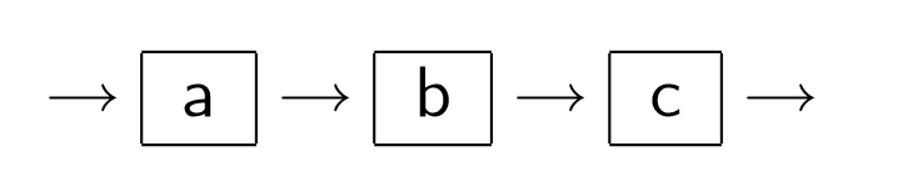
\includegraphics[scale=0.5]{Series.png}
\end{figure}
$$P(\text{System works}) = P(A \cap B \cap C) =P(A)P(B)P(C) = 0.95^3 = 0.857$$


Now calculate the reliability of the system:
\begin{figure}[ht!]
\centering
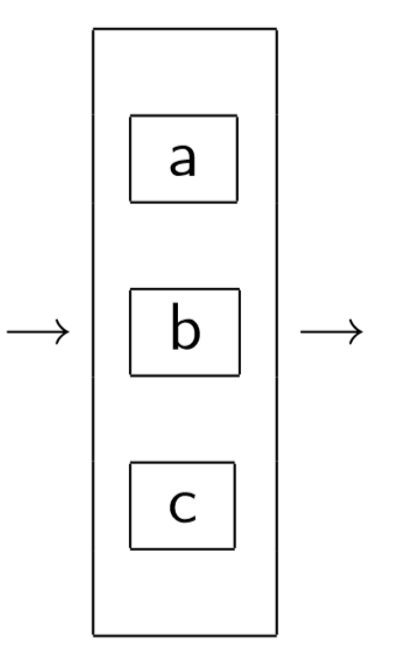
\includegraphics[scale=0.5]{Parallel.png}
\end{figure}
\begin{align*}P(\text{System works}) & = 1- P(\text{System fails}) \\
& = 1 - P(\overline{A} \cap \overline{B} \cap \overline{C}) \\
& = 1 - P(\overline{A})P( \overline{B} )P( \overline{C}) \\
& = 1 - (1-0.95)^3 \\
& = 0.99988 
\end{align*}

\ex

\subsubsection*{Example}

Now suppose$P(A) = P(B) = P(C) = P(D) = 0.95$, calculate the reliability of the system: \begin{figure}[ht!]
\centering
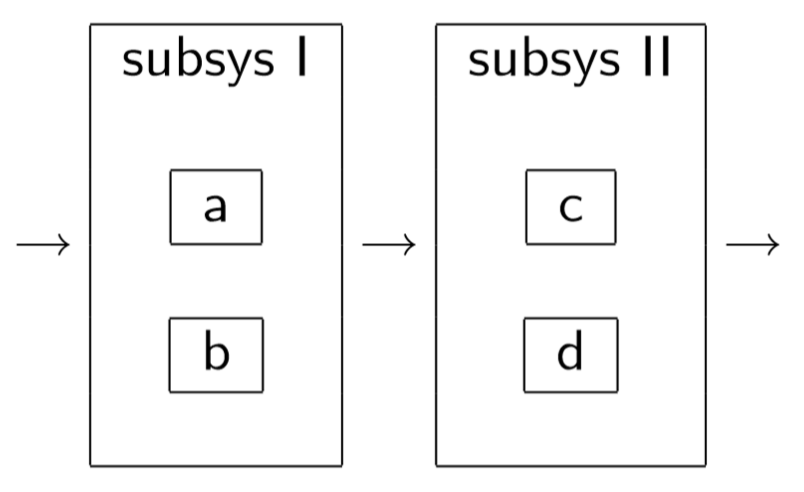
\includegraphics[scale=0.5]{Subs.png}
\end{figure}

\begin{align*}
P(\text{System works}) & = P(\text{Subsys I works} \cap \text{Subsys II works}) \\
& = P(\text{Subsys I works}) P(\text{Subsys II works}) \\
& = (1-P(\overline{A} \cap \overline{B})) (1-P(\overline{C} \cap \overline{D}))\\
& = (1-0.5^2) (1-0.5^2)\\
& = 0.99501
\end{align*}

\subsection{Conditional Independence}

Events $T_1$, $T_2$, $\dots$ $T_n$ are conditionally independent if: 

For all $1 \leq i_1 < i_2 < \dots < i_k \leq n$ and all $1 \leq k \leq n$
\noteworthy{P(T_{i_1} \cap T_{i_2} \cap \dots \cap T_{i_k} | B) = P(T_{i_1} |B) P(T_{i_2}|B) \dots P(T_{i_k}|B)}{Condition for conditional independence}
Which, similarly to the condition for independence of multiple events, say where $n=3$, the  following by itself is insufficient: $$P(T_1 \cap T_2 \cap T_3 |B) = P(T_1|B) P(T_2|B) P(T_3|B)$$ The following are also required conditions: $$P(T_1 \cap T_2 |B) = P(T_1|B) P(T_2|B)$$ $$P(T_1 \cap T_3 |B) = P(T_1|B) P(T_3|B)$$ $$P(T_2 \cap T_3 |B) = P(T_2|B) P(T_3|B)$$ 

Note here that mathematically, conditional independence \textit{does not} imply unconditional independence and vice-versa. However, in practice this can usually be assumed even though there exist counterexamples. So in this course:

If there is conditional independence on $B$, you may assume conditional independence on $\overline{B}$.

We will use this this assumption in developing the sequential Bayes' formula.

\subsection{Sequential Bayes' Formula}

Let $S_i$ be the outcome of the $i$th test, where the outcome can either be positive or negative.

Let $I_k$ be $S_1 \cap S_2 \cap \dots \cap S_k$, ie. the summary of information available after test $k$. Also let $P(E)$ be the probability that part is positive (so the part is defective).

Then set: \begin{align*}
\pi_0 & = P(E)  \\
\pi_1 & = P(E|I_1) = P(E|S_1) \\
\pi_2 & = P(E|I_2) = P(E|S_1 \cap S_2) \\
\pi_3 & = P(E|I_3) = P(E|S_1 \cap S_2 \cap S_3) 
\end{align*}
And so on. Assume that $S_1$, $S_2$, $\dots$, $S_n$ are conditionally independent on $E$ and $\overline{E}$. 

Then for $k = 1,2, \dots, n$:

\noteworthy{\pi_k = \frac{P(S_k|E) \pi_{k-1}}{P(S_k|E) \pi_{k-1} + P(S_k|\overline{E})(1-\pi_{k-1})}}{Bayes' Updating Probability Formula}

Note that this is an iterative process, whereby $\pi_k$ is calculated from $\pi_{k-1}$.

In pseudo-code, the computation would look something like this: \begin{verbatim}
S  = (1, 0, 1, 0...) // test results
n  = n               // number of tests
pi =                 // probability of a defect

pi[0] = pi

for k=1 to n:

   if S[k] == 1: 
       a = p[k]
       b = q[k]
   
   if S[k] == 0:
       a = 1 - p[k]
       b = 1 - q[k]
       
   pi[k] = a*pi[k-1] / ( a*pi[k-1] + b(1-pi[k-1] )
\end{verbatim}

// todo: insert spam example 56/61 here


\section{Random Variables}

The first point to note here is that random variables is a bad name. These are not variables, they're functions.

A random variable, denoted by an upper-case letter, is a function defined on the sample  space to the reals: $$X: \Omega \rightarrow \mathbb{R}$$. 
Where the input is the resulting event from sample space, $\omega$, and the possible value $X$ is a real number, the lower-case letter, $x$.
$$X(\omega) = x$$

For instance, consider the experiment flipping a coin 10 times:
\begin{enumerate}
\item The sample space $\Omega$ is all possible sequences of ten heads  and tails.
\item The outcome $\omega$ could be the possible result $(HTTHHTTTHT)$.
\item The random variable $X$ could be defined as the number of heads in the outcome, and so $X(\omega) = 4$.
\item The random variable $Y$  could be defined as the largest run of tails in the outcome, and so $Y(\omega) = 3$.
\end{enumerate}


The event: "the random variable $X$ takes the value $x$" is mathematically represented as $X=x$, which means \{$\omega: X(\omega) = x$\}. 

This is used for probabilities, where we could say $P(x = X)$ for $x>5$ where the event is that the outcome of the random variable $X$ is greater than 5, and here we can compute the probability of this event.

\subsection{Discrete Random Variables}

A random variable is discrete when its range is either \textit{finite}, such as \{0,1,2,$\dots$,100\}, or \textit{countable} (as in denumerable/countably infinite), such as \{1,2,3,$\dots$\}.

\subsubsection{Probability Mass Function (pmf)}

The \textit{pmf} of a discrete random variable $X$ gives the probability of occurance for each possible value $x$ of $X$. Denoted by a lower-case function letter.
\noteworthy{f(x) = P(X=x)}{pmf}

Properties of the pmf:
\begin{enumerate}
\item $0 \leq f(x) \leq 1$
\item $\sum f(x) = 1$
\item $P(X \in A) = \sum {x \in A} f(x)$ --- if $X$ is a subset of real numbers, then the probability of that equals the sum of those $f(x)$
\end{enumerate}

\subsubsection{Cumulative Distribution Function (cdf)}

Usually just called the distribution function, this is the probability that a random value is less or equal to a given value, denoted by an upper-case function letter.

\noteworthy{F(x) = P(X \leq x) = \sum_{k \leq x} f(k)}{cdf}

\begin{enumerate}
\item $0 \leq F(x) \leq 1$
\item $F(x)$ is non-decreasing
\item $F(-\infty) = 0$, $F(\infty=1)$
\item $P(a < X \leq b) = F(b) - F(a)$
\item $f(k) = F(k) - F(k-1)$
\end{enumerate}

\subsubsection*{Example}

Say the following cdf and pmf are given by the table: \begin{table}[ht!]
\centering
\begin{tabular}{ccc}
\toprule
$x$ & $f(x)$ & $F(x)$ \\
\midrule
0 & 0.15 & 0.15 \\
1 & 0.25 & 0.40 \\
2 & 0.30 & 0.70 \\
3 & 0.20 & 0.90 \\
4 & 0.10 & 1.00 \\
\bottomrule
\end{tabular}
\end{table}

What is the value for $P(1 < X \leq 3)$? $P(1 \leq X < 3)$?

\ex

$$P(1 < X \leq 3) = F(3) - F(1) = 0.90 - 0.40 = 0.50$$
With, $P(1 \leq X < 3)$, note that our cdf properties have the $\leq$ as the upper-bound. But since we know these values are discrete, we can convert the inclusion-exclusion form to an exclusion-inclusion form:
$$P(1 \leq X < 3) = P(0 < X \leq 2) = F(2) - F(0) = 0.70 - 0.15 = 0.55 $$

//todo: example 20/97, and 21/97

\subsubsection{Expected Value}

This is another kind of misleading name, really this is the mean. For instance, if our options are \{0,1,2,3,4\} and they are all equally possible, the expected value is 3.5 but we will never actually expect this value. 

The expected value of a random variable $X$ is denoted as $E(g(X))$, where it is the weighted average of the function $g(X)$.

$$E(g(X)) = \sum_{x} g(x) f(x) $$

The more likely values of $g(x)$ have larger values of $f(x)$ and thus have more weight. Since $E(g(x))$ is considered a "typical value" of $g(x)$, it can be used to summarized $g(X)$.

\subsubsection{Law of Large Numbers}

The law of large numbers merely states that as the number of events increases to infinity, the average value goes to the expected value.

\noteworthy{\text{As } n \rightarrow \infty,\ \ \ \ \ \text{Avg}(X) = \frac{1}{n}(X_1 + X_2 + \dots + X_n) \rightarrow E(X)}{Law of Large Numbers}

This should be fairly obvious. The longer you flip a coin, the more likely it is the number of heads will be approximately equal to the number of tails.

\subsubsection{Linear Operator}

The expected value operator $E$ is a linear operator, meaning that it has a distributive quality, whereby: $$E(X + Y) = E(X) + E(Y)$$
This means that it does not depend on the probability distributions for $X$ and $Y$.

Additionally, constants can be factored out of the operator, and therefore the $E$ of a constant is just the constant: \begin{align*}
E(a + bX) & = E(a) + E(bX) \\
& = aE(1) + bE(X) \\
& = a + bE(X)
\end{align*}


\subsubsection{Moments}

\subsubsection{Mean, Variance, Standard Deviation}

Mean: \noteworthy{\mu = E(X) = \sum x f(x)}{Mean from pmf}
Variance: \noteworthy{\sigma^2 = \text{Var}(X) = E \br{(X-\mu)^2} = \sum (x-\mu)^2 f(x)}{Variance from pmf}
Standard deviation: $$ \sigma = \sqrt{ \sum (x-\mu)^2 f(x) }$$

When calculating the variance by hand, you can use: \noteworthy{ \sigma^2 = E(X^2) - E(X)^2 = \mu_2 - \mu^2 }{Variance approximation}

\subsubsection*{Example}

Take the following table: \begin{figure}[ht!]
\centering
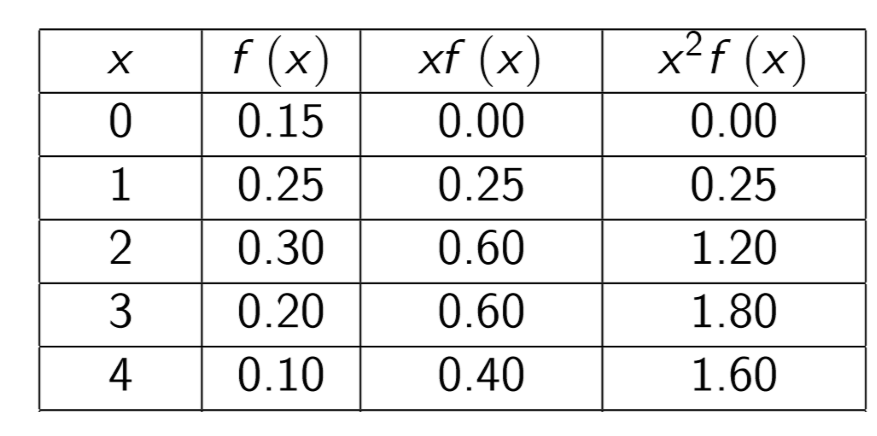
\includegraphics[scale=0.5]{T1.png}
\end{figure}

Calculate the mean, standard deviation, and variance.

\ex

Mean: $$\mu = E(X) = \sum x f(x) = 0.25 + 0.60 + 0.60  + 0.40 = \boxed{1.85}$$

$$\mu_2 = \sum x^2 f(x) = 0.25 + 1.20 + 1.80 + 1.60 = 4.85 $$
Variance: $$\sigma^2 = \text{Var}(X) = \mu_2 - \mu^2 = 4.85 - 1.85^2 = \boxed{1.4275}$$
Standard deviation: $$ \sigma = \sqrt{ 1.4275 } = \boxed{1.1948}$$

\ex

\subsubsection*{Example}

For $x = 1,2, \dots, 10$: $$f(x) = \frac{1}{2.928968} \times  \frac{1}{x}$$ 

Calculate the mean, standard deviation, and variance. 

\ex

$$\mu = \sum x f(x) = \sum_{x=1}^{10} x \frac{1}{2.928968x} = \sum_{x=1}^{10} \frac{1}{2.928968}  =\frac{10}{2.928968} = \boxed{3.4142}$$
$$\mu_2 = \sum x^2 f(x) = \sum_{x=1}^{10} \frac{x}{2.928968}  =\frac{55}{2.928968} = \boxed{18.77855}$$
$$\sigma^2 = \mu_2 - \mu^2 = 18.77855 - 3.4142^2 = \boxed{7.1218}$$
$$\sigma =  \boxed{2.6687}$$

\subsubsection*{Example}

Where the pmf is: $$f(x) = \begin{cases}
(1-p)^2 & x=0 \\
2p(1-p)^2 & x=1 \\
p^2 & x=2 \\
\end{cases}$$

Calculate the expected value, variance, and standard deviation. 

\ex

$$\mu = \sum xf(x) = 0(1-p)^2 + 1(2p(1-p)) + 2(p^2) = 2p(1-p) + 2p^2 = \boxed{2p}$$
$$\mu_2 = \sum x^2 f(x) = 0(1-p)^2 + 1(2p(1-p)) + 4(p^2) = 2p(1-p) + 4p^2 = 2p + 2p^2$$
$$\sigma^2 = \mu_2 - \mu^2 = (2p+2p^2) - (2p)^2 = \boxed{2p -2p^2}$$
$$\sigma =  \boxed{\sqrt{2p -2p^2}}$$

\ex 

\subsubsection*{Example}

An urn contains $n$ chips numbered 1 through $n$. We draw $k$ chips (1<$k$<$n$) without replacement. Let $Y$ represent the highest number among those drawn. \begin{enumerate}[(a)]
\item What is the range of $Y$?
\item Find $F_Y(y)$
\item Find $f_Y(y)$
\item Suppose $n=20$ and $k=5$. Calculate the mean, variance, and standard deviation for $Y$.
\end{enumerate}

\ex

(a) Suppose the first selection was the smallest possible value, 1. Then the value of $Y$ would be 1. Then for the second selection, the next smallest value would be 2. This would continue, and so because there is no replacement, the smallest possible value for $Y$ is the $k$th chip. The largest possible selection is $n$. So the range is $\boxed{\{k,k+1, \dots, n\}}$.

(b) $F(y)$ is 

(c) $f(y)$ is

(d)

//todo

\subsubsection{Properties of the Mean}

The mean minimizes the Mean Square Error: $$ S(t) = E[X-t)^2] \geq E[(X - \mu)^2] = \text{Var}(X), \ \ \ \, \text{for all } t$$

\begin{proof}
Recall that $E(a + bX) = a + bE(X)$ for constants $a$, $b$.
\begin{align*}
S(t) & = E(X^2 + t^2 - 2Xt) \\
& = E(X^2) + t^2 - 2\mu t \\
S'(t) & = 2t-2\mu = 0 \implies t = \mu \\
S''(\mu) & = 2 > 0 \ \ \ (\mu\ \text{is a minimizer})
\end{align*} \end{proof}
\subsubsection{Properties of the Variance}

\begin{align*}
Var(a + bX) & = E[a + bX - E(a + bX) ]^2 \\
& = E[a + bX -a - E(bX) ]^2 \\
& = E[bX - bE(X) ]^2 \\
& = E[b^2(X - E(X))^2 ] \\
& = b^2 E[(X - E(X))^2 ] \\
& = b^2 Var(X)
\end{align*}

Therefore: \noteworthy{Var(a + bX) = b^2 Var(X)}{Property of Variance}

Additionally: $$\text{StdDev}(a + bX) = |b|\text{StdDev}(X)$$


\subsubsection{Binomial Random Variables}

Let $A$ be an occurrence we want to monitor. We'll call the occurrence  of $A$ a success, and the non-occurrence a failure, and $p=P(A)$ where $p$ is the probability of success

The number of instances of $A$ that are monitored (\textit{independent} trials) is $n$, where the outcome could either be a success or a failure. The number of successes is: $$X \sim Bin(n,p)$$

The range of $X$ is zero to the number of possible successes: $$\text{Range} = \{0,1,2, \dots, n\}$$

The density of a \textbf{binomial random variable} is (assumes independence): \noteworthy{P(X = x) = f(x) = {n \choose x} p^x (1-p)^{n-x},\ \ \ \ \ x = 0,1,2, \dots, n}{cdf of a Binomial Random Variable}

Recall where: $${n \choose x} = \frac{n!}{x!(n-x)!}$$

This is a random variable, so it has a moment-generating function (??? get clarity of moment generating functions): $$M(t) = (1-p + pe^t)^n$$ 
$$M'(t) = \deriv{}{t}{M(t)} = n(1-p+pe^t)^{n-1} pe^t$$
$$M''(t) = n(n-1)(1-p+pe^t)^{n-1} p^2e^{2t} + n(1-p+pe^t)^{n-1} pe^t$$

The mean, $\mu = M'(0) = n(1-p+pe^0)^{n-1}pe^0 = np$, and so the mean is the number of trials multiplied by the probability of success: \noteworthy{\mu =  M'(0) = E(X) = np} {Mean of a Binomial Random Variable}

And: $$\mu_2 = n(n-1)p^2 + np$$

The variance is $\sigma^2 = M''(0) - M'(0)^2 = \mu_2 - \mu^2$: \noteworthy{\sigma^2 = np(1-p)}{Variance of a Binomial Random Variable}
Note that the variance is maximized where $p=0.5$, because if $p=0.9$, there are mostly successes and if $p=0.1$, there are mostly failures.

\subsubsection*{Example}

Suppose that finding oil when digging at certain locations has a probability $p=0.10$ (geologically determined locations).
\begin{enumerate}[(a)]
\item How many wells should we dig to find oil with probability larger than or equal to 0.95?
\item How many wells should we dig to obtain at least 2 successful wells with probability larger than or equal to 0.95?
\end{enumerate}

\ex

Assume that each well is independent, then $ X \sim Bin(n, 0.10)$ is the number of wells with oil where $n$ is the number of dug wells.
\begin{enumerate}[(a)]
\item The probability of finding oil is $P(X > 0)$. 
\begin{align*}P(X > 0) & = 1 - P(X = 0) \\
& = 1 - {n \choose 0} p^0 (1-p)^{n-0} \\
& = 1 - (1 - 0.10)^n \\
& = 0.95 
\end{align*}
Solving for $n \rightarrow n = 28.43$, so must dig at least $\boxed{29}$ wells.

\item \begin{align*}
0.95 & = P(X \geq 2) \\
& = P(X > 1) \\
& = 1 - P(X = 1) - P(X = 0) \\
& = 1 - \br{{n \choose 1} p^1 (1-p)^{n-1}} - \br{{n \choose 0} p^0 (1-p)^{n-0}}  \\
& = 1 -  \br{n 0.10 (1-0.10)^{n-1}} - (1-0.10)^{n}
\end{align*}
Solving for $n \rightarrow \boxed{n = 49}$.

\end{enumerate}


\subsubsection{Poisson Random Variables}

Let's say we want to count the number of occurrences of  certain event $A$, that has a typical rate of occurrences per time period (or per area), $\lambda$. The quantity of interest is $X$, the number of occurrences.
$$X \sim \mathcal{P}(\lambda)$$

For a \textbf{Poisson random variable} is, the probability of $k$ occurrences in the interval [0,$t$] is written as: $$P(k; t)$$ 

With Poisson random variables we make the following assumptions: \begin{enumerate}
\item Occurrences in disjoint time intervals are independent
\item There is \textbf{proportionality}, meaning: $$P(1;t) = \lambda t + o(t), \ \ \ \text{where} \lim_{t\rightarrow0} \frac{o(t)}{t} = 0$$

Here, $o(t)$ represents the order, and this means that $o(t)$ goes to zero faster than $t$.  (??? what's the significance of this?)

\item Events are \textbf{rare events}, meaning that events are sparse and have at most 1 occurrence of $A$ in a  small period of time: $$1-P(0;t) - P(1;t) = \sum_{k=2}^{\infty} P(k;t) = o(t)$$
\end{enumerate}

For Poisson, $X$ represents the number of occurrences over the range $\{0,1,2,\dots\}$

The pmf of a Poisson: \noteworthy{f(x) = P(X=x) = \frac{e^{-\lambda}\lambda^x}{x!}, \ \ \ \ \ \ x = 0, 1, 2, \dots}{pmf of Poisson Random Variable}

The moment generating function: $$M(t) = e^{\lambda(e^t -1 )}$$ 

The mean: \noteworthy{\mu = M'(0) = E(X) = \lambda}{Mean of Poisson Random Variable}

And the variance: \noteworthy{\sigma^2 = M''(0) - M'(0)^2 = Var(X) = \lambda}{Variance of Poisson Random Variable}

Note that with a Poisson random variable, $\mu = \sigma^2 = \lambda$. When looking at real data, if your mean and variance are very close and events can be considered rare, you might be able  to model your system with the Poisson distribution -- if not, it could be overly or underly spaced and you cannot use Poisson.

\subsubsection*{Example}

Suppose that the number of earthquakes over 5.0 on the Richter scale in a given area is a Poisson random variable and there are on average 3.6 of these earthquakes per year.

\begin{enumerate}[(a)]
\item What is the probability of having at least 2 earthquakes over 5.0 during the next 6 months?
\item What is the probability of having 1 earthquake over 5.0 next month?
\item What is the probability of waiting more than 3 months for the next earthquake over 5.0?
\end{enumerate}

\ex

We know: $$Y \sim \mathcal{P}(\lambda)$$ 
And $\lambda$ = 3.6/year = 0.3/month = 1.8/(6-months) = 0.9/(3-months)

\begin{enumerate}[(a)]
\item The probability of having at least two earth quakes in the next six months, here we use the $\lambda$ = 1.8/(6-months) to keep the interval consistent.
\begin{align*}
P(X \geq 2) & = P(X > 1) \\
& = 1 - P(X=1) - P(X = 0) \\
& = 1 - \frac{e^{-\lambda}\lambda^1}{1!} - \frac{e^{-\lambda}\lambda^0}{0!}\\
& = 1 - 1.8e^{-1.8} - e^{-1.8} = \boxed{0.53716}
\end{align*}
\item Here we use $\lambda=0.3$/month. \begin{align*} 
P(X = 1) & =  \frac{e^{-\lambda}\lambda^x}{x!} = \frac{e^{-0.3}0.3^1}{1!} = \boxed{0.22225}
\end{align*}
\item  The probability of waiting more than three months is the same as the probability that there are no earthquakes in a rate of \# earthquakes per three months, so $\lambda = 0.9$/month. \begin{align*} 
P(\text{Waiting > 3 months}) & =  P(X = 0) \\
& = \frac{e^{-\lambda}\lambda^x}{x!} \\
& = \frac{e^{-0.9}0.9^0}{0!} = \boxed{0.40657} 
\end{align*}
\end{enumerate}

Poisson random variables are memoryless, so it doesn't matter where we start. The probability that no earthquakes happen in the next three months is the same as the probability that no earthquakes happen in the three months after that, and so on.








\subsection{Continuous Random Variables}

A random variable is continous when its range is an interval, such as (0,1). 

\subsubsection{PDF and CDF}

Some properties of the density of a continuous random variable are the following: \begin{enumerate}
\item The function is non-negative: $$ f(x) \geq 0$$
\item The function integrates to one: $$ \int_{-\infty}^{\infty} f(x) dx = 1 $$
\item The integral of a range can be used to compete probabilities: $$P(a < X < b) = \int_a^b f(x) dx$$
\end{enumerate}

Some  properties of the distribution function of a continuous random variable are the following:
\begin{enumerate}
\item The probability of a value greater than a given $x$ is the cdf: \noteworthy{F(x) = P(X \leq x) = \int_{-\infty}^{x} f(t) dt}{cdf of continuous random variable}
\item The cdf can be used to compute the probability of a range $P(a < X < b)$. Because $\int_{a}^b f(x) dx = \int_{-\infty}^b f(x) dx - \int_{a}^\infty f(x) dx$, we can show: \noteworthy{P(a < X < b) = \int_{a}^b f(x) dx = F(b) - F(a)}{Probability of range of continuous random variable}
 Here the probability is the difference between the area under the upper limit of the curve minus the area under the lower limit of the curve. 
 
 Note that it doesn't matter whether the inequalities are $<$ or $\leq$ because as equation (\ref{Probability of exact value with continuous random variable}) shows, $P(X = a) = P(X = b) = 0$, so: $$P(a < X < b) = P(a \leq X \leq b)$$
\end{enumerate}

\textbf{Note:} Although for discrete random variables, we had $f(x) = P(X = x)$, but this is not true of continuous random variables. For continuous random variables: \noteworthy{P(X = x) = \int_x^x f(t) dt = 0, \ \ \ \  \ \ \text{for all x}}{Probability of exact value with continuous random variable} And so $f(x) \neq P(X = x)$. In fact, we often have $f(x) > 1$. However, for a very small $\delta > 0$, we can approximate: $$ P(x < X < x + \delta) = \int_x^{x+\delta} f(t) dt \approx f(x) \delta $$

Also, note that: \noteworthy{F'(x) = \deriv{}{x}{\int_{-\infty}^x f(t) dt}= f(x)}{pdf from cdf of continuous random variable}


\subsubsection{Mean and Variance}

\noteworthy{\mu = \int_{-\infty}^{\infty} x f(x) dx}{Mean of continuous random variable}

\noteworthy{\var = \int_{-\infty}^{\infty} (x - \mu)^2 f(x) dx = \int_{-\infty}^{\infty} x^2 f(x) dx - \mu^2 = \mu_2 - \mu^2}{Variance of continuous random variable}

\subsection{Uniformly Distributed Random Variables}

Uniform random variables are probably the simplest there are. Here, everything has the same density on a given interval, so each value in the interval has the same probability. This is very powerful in simulation.

The notation for a uniform random variable, where $\alpha$ is the lower limit and $\beta$ is the upper limit, is: $$ X \sim Unif(\alpha, \beta) $$

\subsubsection{PDF and CDF}

The probability density function of a uniform random variable visually looks like a horizontal line, and is defined as: \noteworthy{f(x) = \begin{cases} 
0 & x \leq \alpha \\ 
(\beta-\alpha)^{-1} & \alpha < x < \beta \\ 
0 & x \geq \beta 
\end{cases}}{pdf of uniform random variable}

And the distribution function visually looks like a linear increase from $\alpha$ to $\beta$, and is 0 before and 1 after. It is defined as: 
\noteworthy{F(x) = \int_\alpha^x f(t) dt = \begin{cases} 
0 & x \leq \alpha \\ 
(x-\alpha)/(\beta-\alpha)  & \alpha < x < \beta \\ 
1 & x \geq \beta 
\end{cases}}{cdf of uniform random variable}

But from now on we'll ignore the domain $x \leq \alpha$ and $x \geq \beta$, and so: \noteworthy{P(a < X < b) = F(b) - F(a) = \frac{b-a}{\beta - \alpha}}{Probability of range of uniform random variable}


When you are told for example that $X ~ \sim \text{Unif}(0, 1)$, this means:  $$f_X(x) = 1 \ \ \ \ \ \text{for}\ 0 \leq x \leq 1 $$ $$F_X(x) = x \ \ \ \ \ \text{for}\ 0 \leq x \leq 1 $$

\subsubsection{Mean and Variance}

The mean of a uniform random variable is simply the average of the upper and lower limit: \noteworthy{\mu = \frac{1}{\beta-\alpha} \int_{\alpha}^\beta x dx = \frac{\alpha + \beta}{2}}{Mean of a uniform random variable}
And the second mean is: $$\mu_2 = \frac{1}{\beta-\alpha} \int_{\alpha}^\beta x^2 dx = \frac{\beta^2 + \alpha^2 + \alpha\beta}{3}$$
And so the variance is: \noteworthy{\var = \mu_2 - \mu^2 = \frac{(\beta - \alpha)^2}{12}}{Variance of uniform random variable}

\subsubsection*{Example}
Suppose that $X$ is Unif(0, 10). Calculate $P(X>3)$ and $P(X > 5|X >2)$.

\ex

So $\alpha = 0$, $\beta=10$, and $x=3$.

\begin{align*}
P(X > 3) & = 1 - F(3) \\
& = 1 - \frac{x-\alpha}{\beta-\alpha} \\
& = 1 - \frac{3-0}{10 - 0}  = \boxed{0.7} \\
\end{align*}

Now $\alpha = 0$, $\beta=10$, and $x=5$.

\begin{align*}
P(X > 5 | X > 2) & = \frac{P(X>5 \cap X>2)}{P(X>2)} \\
& = \frac{P(X>5)}{P(X>2)} & \text{In order for both to be true,}\ X>5 \\
& = \frac{1 - F(5)}{1 - F(2)} \\
& = \frac{1 - \frac{5-0}{10-0}}{1 - \frac{2-0}{10-0}} = \boxed{0.625} \\
\end{align*}


\subsubsection*{Example}

Suppose that $X$ is Unif(0,1). Derive the distribution function and density function for $Y = -\ln(X)$. 

\ex

Since $X$ is Unif(0,1), then:  $$ f_X(x) = 1,\ 0 \leq x \leq 1 $$ $$ F_X(x) = x,\ 0 \leq x \leq 1 $$

Notice that the range of $Y$ is $(0, \infty)$, so for $y < 0$: $$ F_Y(y) = 0$$


\ex

For $y > 0$: \begin{equation} 
\begin{split} F_Y(y) & =  P(Y \leq y) \\ 
& = P( -\ln(X) \leq y)  \\
& = P(X \geq e^{-y}) \\
& = 1 - F_X(e^{-y}) \\ 
& = \boxed{1 - e^{-y}} 
\end{split} 
\end{equation}

Similarly, for $y > 0$: $$ f_Y(y) = F'_Y(y) = \frac{\partial}{\partial y} (1- e^{-y}) = \boxed{e^{-y}} $$

\subsection{Exponential Random Variables}

Exponential random variables are used to model the waiting time until the occurrence of a certain event. Exponential density functions have the input rate of occurrence, $\lambda$ = \# of occurrences/time intervals,  and the notation for an exponential random variable is: $$X \sim Exp(\lambda)$$

\subsubsection{PDF and CDF}

The density function for an exponential random variable is: \noteworthy{f(x) = \begin{cases} \lambda e^{-\lambda x} & x > 0 \\ 0 & \text{otherwise} \end{cases}}{pdf for exponential random variable}

And similarly for $x \leq 0$, $F(x) = 0$. For $x>0$, the distribution function is: \noteworthy{P(X \leq x) = F(x) =  \int_0^x e^{-\lambda t} dt  = 1- e^{-\lambda x}}{cdf for exponential random variable}

\subsubsection{Mean and Variance}

The mean of an exponential random variable is: \noteworthy{\mu = \frac{1}{\lambda}}{Mean of exponential random variable} And the variance: \noteworthy{\var = \frac{1}{\lambda^2}}{Variance of exponential random variable}

Note that: \noteworthy{Exp(\lambda) = \frac{-\ln{(Unif(0,1))}}{\lambda}}{Exponential from uniform random variable}

Note that exponential random variables are memoryless, so they have a constant probability.  Where $X \sim Exp(\lambda)$: $$P(X > h) = P(X > h+x\ |\ X > x) =    e^{-\lambda h} $$ So at age $x$, the probability of surviving $h$ additional units is the same for all ages $x$.

\subsubsection{Failure Rate}

\noteworthy{\lambda(x) = \frac{f(x)}{1-F(x)} = - \deriv{}{x}{\ln[1-F(x)]}}{Failure rate}

If the failure rate increases, it means the system wears out over time. Exponential random variables are the only type of random variable in the continuous domain that have a constant failure rate. $$\lambda(x) \delta \approx P(X \leq x + \delta\ |\ X > x), \ \ \ \ \ \ \ \text{for a small}\ \delta $$

Given the failure rate, from (\ref{Failure rate}), we can calculate the distribution function: \noteworthy{F(x) = 1 - e^{-\int_0^x \lambda(t) dt}}{cdf from failure rate}

For a constant failure rate, where $\lambda(x)=k$: $$ F(x) = 1 - e^{-kx} $$

An increasing failure rate is often used in engineering. For instance, the Weibull distribution is where $\lambda(x) =x$ and is often used to demonstrate where there is a linear increase in failure rate: \noteworthy{F(x) = 1 - e^{-\frac{1}{2}x^2}}{Weibull distribution}

For a decreasing failure rate, for example where $\lambda(x) = \frac{1}{1+x}$:  $$F(x) = 1 - e^{-\int_0^x \frac{1}{1+t} dt} = 1 - e^{-[\ln{(x+1) - \ln{(1)]}}}= 1 - \frac{1}{x+1} = \frac{x}{x+1} $$

\subsection{Normal Distribution}

\subsubsection{Standard Normal Distribution}

The standard normal random variable is denoted by $Z$. The standard normal density is where $\mu=0$ and $\var=1$: \noteworthy{\varphi(z) = \frac{1}{\sqrt{2\pi}} e^{-\frac{1}{2}z^2}}{Standard normal density function}

Standard normal distribution function: \noteworthy{P(Z \leq z) = \Phi(z) = \int_{-\infty}^z \varphi(t) dt}{Standard normal distribution function}

$\Phi(z)$ cannot be calculated in closed form, meaning it can't be calculated in a finite number of operations, so you'll usually either look it up in a table or use a computer, such \verb|pnorm(z)| in $R$. The normal density function is symmetrical, therefore: \noteworthy{\Phi(z) = 1 - \Phi(-z)}{Symmetry formula} \noteworthy{\mu = E(Z) = \int_{-\infty}^{\infty} z \varphi(z) dz = 0}{Mean of standard normal distribution} \noteworthy{\var = Var(Z) = \int_{-\infty}^{\infty} z^2 \varphi(z) dz = 1}{Variance of standard normal distribution}

\subsubsection{General Normal Random Variables}

The notation for a normal random variable is: $$X \sim N(\mu, \var)$$

You can create a non-standard normal distribution with measurements $X_1$, $X_2$, $\dots$, $X_n$ from a standard normal distribution $Z_1$, $Z_2$, $\dots$, $Z_n$, where: $$ X_i = \mu + \sigma Z_i \ \ \ \ \ \ \ i =1,2,\dots,n $$ 

And because $E(Z)=0$ and $Var(Z)=1$ for the standard normal variable $Z$: $$\boxed{E(X) = E(\mu + \sigma Z) = \mu + \cancelto{0}{\sigma E(Z)} = \mu}$$ $$\boxed{Var(X) = Var(\mu + \sigma Z) = \sigma^2 \cancelto{1}{Var(Z)} = \var}$$

The distribution function for $X$ is: \begin{align*}
F(x) & = P(X \leq x) \\ 
& = P \br{ \frac{X-\mu}{\sigma} \leq \frac{x-\mu}{\sigma} } \\
& = P \br{ Z \leq \frac{x-\mu}{\sigma} }  \end{align*} \noteworthy{F(x) = \Phi \br{\frac{x-\mu}{\sigma}}}{cdf of normal random variable}

The density function for $X$ is: \noteworthy{f(x) = F'(x) = \frac{1}{\sigma\sqrt{2\pi}} e^{-\frac{1}{2}\br{\frac{x-\mu}{\sigma}}^2}}{pdf of normal random variable}


\subsubsection*{Example}

Let $Z \sim N(0, 1)$ and calculate: \begin{enumerate}[(a)]
\item $P(0.10 \leq Z \leq 0.35)$
\item $P(Z > 1.25)$
\item $P(Z > -1.20)$
\item Find $c$ such that $P(Z > c) = 0.05$
\item Find $c$ such that $P(|Z| < c) = 0.95$
\end{enumerate} 

\ex

\begin{enumerate}[(a)]
\item \begin{align*}
P(0.10 \leq Z \leq 0.35) & = \Phi(0.35) - \Phi(0.10) = \boxed{0.0970}
\end{align*}
\item \begin{align*}
P(Z > 1.25) & = 1 - P(Z \leq 1.25) \\ 
& = 1 - \Phi(1.25) = \boxed{0.1056}
\end{align*}
\item  \begin{align*}
P(Z > -1.20) & = 1 - P(Z \leq -1.20) \\ 
& = 1 - (1-\Phi(1.20)) = \boxed{0.8849}
\end{align*}
\item Find $c$ such that $P(Z > c) = 0.05$ \begin{align*}
P(Z > c) & = 0.5 \\
1 - P(Z \leq c) & = 0.5 \\
 P(Z \leq c)  & = 0.95 \\
 \Phi(c) & = 0.95  \\ 
c  & = \Phi^{-1}(0.95)  = \boxed{1.644854}
\end{align*}
\item Find $c$ such that $P(|Z| < c) = 0.95$
\begin{align*}
P(-c < Z < c) & = 0.95 \\
\Phi(c) - \Phi(-c) & = 0.95 \\
\Phi(c) - (1-\Phi(c)) & = 0.95 \\
2\Phi(c) & = 1.95 \\
c & = \Phi^{-1}\br{\frac{1.95}{2}} = \boxed{1.959964}
\end{align*}
\end{enumerate} 

\subsubsection{Summary}

\begin{table}[H]
\centering
\caption{Summary of Probability Distribution Models}
\small
\begin{tabular}{lll}
\toprule
 \textbf{What we know} & \textbf{What to determine} & \textbf{What model to use} \\
 \midrule
 Occurrences with a probability of success & Number of successes & Binomial \\
  Rate of occurrence & Number of occurrences & Poisson \\
   &  & Uniform \\

  Rate of occurrence  & Waiting time until occurrence & Exponential \\

  \bottomrule
\end{tabular}
\end{table}


\section{Random Vectors}

\subsection{Continuous Random Vectors}

$X_1$ and $X_2$ are random variables, that may or may not be independent. 
$$\text{Random vector},\ X = {X_1 \choose X_2}$$

Random vectors also have pdf, called \textit{joint pdf} or \textit{joint density}. 
$$f_{X1,X2} (x1, x2)$$

Properties of joint pdf:

\begin{itemize}
\item Non-negative -- $f_{X1,X2} (x1, x2) \geq 0$ for all $x_1 \in R$ and $x_2 \in R$
\item $$\int_{-\infty}^\infty\int_{-\infty}^\infty f_{X1,X2} (x1, x2) dx_1 dx_2 = 1$$
\end{itemize}

Joint cdf, $F_{X_1, X_2}(x_1, x_2)$:

\begin{itemize}
\item $$F_{X_1, X_2}(x_1, x_2) = P(X_1 \leq x_1, X_2 \leq x_2) = \int_{-\infty}^{x_2}\int_{-\infty}^{x_1} f_{X1,X2} (t_1, t_2) dt_1 dt_2 $$

\item $$\frac{\partial^2}{\partial x_1 \partial x_2} F_{X_1, X_2} (x_1, x_2) = f_{X_1, X_2}(x_1, x_2)$$
\end{itemize}

\subsubsection{Dependence and Independence}

If and only if $X_1$ and $X_2$ are independent, then $$f_{X_1, X_2}(x_1, x_2) = f_{X_1}(x_1)f_{X_2}(x_2)$$

Expectation and variance-covariance matrix:

$$E  {X_1 \choose X_2}  == {E(X_1) \choose E(X_2)} = {\mu_1 \choose \mu_2}$$

$$ \Sigma = Cov{X_1 \choose X_2} = \begin{bmatrix}
\text{Cov}(X_1, X_1) & \text{Cov}(X_1, X_2) \\
\text{Cov}(X_2, X_1) & \text{Cov}(X_2, X_2) \\
\end{bmatrix} = 
\begin{bmatrix}
\text{Var}(X_1) & \text{Cov}(X_1, X_2) \\
\text{Cov}(X_2, X_1) & \text{Var}(X_2) \\
\end{bmatrix}  $$ 


Covariance is $Cov(X_1, X_2) = E(X_1 X_2) - E(X_1) E(X_2)$, so: $$Cov(X_1, X_1) = E(X_1^2) - E(X_1)^2 = Var(X_1)$$

Note that the variance-covariance matrix is symetrial because on the left-to-right diagonal it has variances and on the right-to-left diagonal they're the same.

$$Cov(X1, X2) = E \{(X_1 - E(X_1)(X_2 - E(X_2) \}$$

If the $X_1$ and $X_2$ are independent, $Cov(X_1, X_2) = 0$. But this in \textit{not} a biconditional.

\begin{proof}
$$E(X_1, X_2) = \int_{-\infty}^{\infty}\int_{-\infty}^{\infty} X_1 X_2 f_{X_1, X_2}(x_1, x_2) dx_1 dx_2 $$

$$ = \int_{-\infty}^{\infty}\int_{-\infty}^{\infty} x_1 f_{X_1} (x_1) x_2 f_{X_2} (x_2) dx_1 dx_2$$

$$ = \int_{-\infty}^{\infty} x_1 f_{X_1} (x_1) dx_1\int_{-\infty}^{\infty}  x_2 f_{X_2} (x_2)  dx_2$$

$$=E(X_1) E(X_2) = Cov(X_1, X_2) = E(X_1, X_2) - E(X_1)E(X_2) = 0$$

Conditional distributions

$$f_{X_1 | X_2 = x_2} (x_1, x_2) = \frac{f_{X_1, X_2}(x_1, x_2)}{f_{X_2}(x_2)}$$

Marginal distributions:

Individual distribution of $x_1$: $$f_{X_1} (x_1) = \int_{-\infty}^{\infty} f_{X_1, X_2} (x_1, x_2) dx_2$$

\end{proof}

\subsection*{Example 1}

$X_1 \sim Unif(0,1)$, $X_2 \sim Unif(0,1)$, $X_1$ and $X_2$ are independent.

$$f_{X_1}(x_1) = \frac{1}{1-0} = 1$$

$$f_{X_2}(x_2) = \frac{1}{1-0} = 1$$

\begin{enumerate}[(a)]
\item Find the joint pdf of $X_1 \choose X_2$

$$f_{X_1, X_2}(x_1, x_2) = 1 \times 1 = 1$$

\item Find the joint cdf:

$$F_{X_1, X_2}(x_1, x_2) = P(X_1 \leq x_1 \cap X_2 \leq x_2) = P(X_1 \leq x_1) P(X_2 \leq x_2) = x_1 x_2$$

In general:
$F_{X_1, X_2}(1, 1) = 1$, $F_{X_1, X_2}(0,0) = 0$, $F_{X_1, X_2}(\infty, \infty) = 1$, $F_{X_1, X_2}(-\infty, -\infty) = 0$.

\item Find $E{X_1 \choose X_2}$:

$$E{X_1 \choose X_2} = {E(X_1) \choose E(X_2)} = {0.5 \choose 0.5}$$

\item Find $Cov(X_1, X_2) = \Sigma$


$$ \Sigma = Cov{X_1 \choose X_2} = 
\begin{bmatrix}
\text{Var}(X_1) & \text{Cov}(X_1, X_2) \\
\text{Cov}(X_2, X_1) & \text{Var}(X_2) \\
\end{bmatrix} =  
\begin{bmatrix}
1/12 & 0 \\
0 & 1/12 \\
\end{bmatrix}
$$ 

Zeros from right-to-left diagonals because $X_1$ and $X_2$ are independent.

\end{enumerate}

\subsection*{Example 2}

Joint pdf $f_{X_1, X_2} = c(x_1^2 + x_2^2)$, where $c$ is the normalization constant and $x_1, x_2 \in [0,1]$

\begin{enumerate}[(a)]

\item Find $c$

$$ 1 = \int_0^1 \int_0^1 c(x_1^2 + x_2^2) dx_1 dx_2 $$
$$  = c \int_0^1 \int_0^1 (x_1^2 + x_2^2) dx_1 dx_2 $$
...
$$  = 2/3(c), \ \ \ \ x_1, x_2 \in [0,1]  $$

So $c$ = 3/2.

$$f_{X_1 X_2} = \frac{3}{2}(x_1^2 + x_2^2) \ \ \ \ \ x_1, x_2 \in [0,1]$$

\item Find joint cdf:

$$F_{X_1X_2} (x_1, x_2) = \int_0^{x_1} \int_0^{x_2} \frac{3}{2}(t_1^2 + t_2^2) dt_1 dt_2 = \frac{x_1^3 x_2 + x_1 x_2^3}{2}, \ \ \ \ \ \ x_1, x_2 \in [0,1]$$

\item Find the marginal pdf and cdf of $x_1$:

$$f_{X_1}(x_1) = \int_0^1 \frac{3}{2} (x_1^2 + x_2^2) dx_2$$

$$=\frac{3}{2} \br{ x_1^2 + \frac{1}{3} }, \ \ \ \ x_1, x_2 \in [0,1]$$

$$F_{X_1}(x_1) = \int_{0}^{x_1} \br{ \frac{3}{2} x_1^2 + \frac{1}{2} } dx_1 = \frac{1}{2} x_1^3 + \frac{1}{2}x_1, \ \ \ \ x_1, x_2 \in [0,1]$$


\item $Cov(X_1, X_2) = E(X_1, X_2) - E(X_1) E(X_2)  $

$$E(X_1, X_2) = \int_0^1 \int_0^1 x_1 x_2 f_{X_1 X_2}(x_1, x_2) dx_1 dx_2  = \int_0^1 \int_0^1 x_1 x_2 \frac{3}{2}(x_1, x_2) dx_1 dx_2 = $$ 

$$E(X_1) = \int_0^1 x_1 f_{X_1} (x_1) dx_1 = \int_0^1 \br{\frac{3}{2}x_1^3 + \frac{1}{2}x_1} dx_1 = \frac{5}{8} $$

$$E(X_2) = E(X_1) = \frac{5}{8}$$

$$Cov(X_1, X_2) = \frac{3}{8} - \br{\frac{5}{8}}^2 = \frac{-1}{64}$$

\end{enumerate}



$X_1$ and $X_2$ could be independent if $f_{X_1 X_2} = x_1 x_2$ because they can be products of their own parts. $f_{X_1 X_2} = x_1 x_2 + x_1$ could also be independent because you can factor it into $f_{X_1 X_2} = x_1(x_2 + 1)$. 

If it's $f_{X_1 X_2} = x_1 x_2 + x_1 + x_2$ then you can't factor them, so they're not independent. 

\subsection{Coorelation}


This defines the strength of linear relationship between $X_1$ and $X_2$:
$$r = \frac{Cov(X_1, X_2)}{\sqrt{Var(X_1)Var(X_2)}} = \frac{E(X_1, X_2) - E(X_1)E(X_2)}{\sqrt{E(X_1^2) - E(X_1)^2} \sqrt{E(X_2^2) - E(X_2)^2}}$$

Correlation can only be between two variables. With more there can only be pairwise correlation.

$$X_1 \text{and} X_2\ \text{are independent} \implies r=0$$

$$X_1 \text{and} X_2\ \text{are independent and jointly normal} \iff  r=0$$

$$ \Sigma_x = 
\begin{bmatrix}
\text{Var}(X_1) & \text{Cov}(X_1, X_2) \\
\text{Cov}(X_2, X_1) & \text{Var}(X_2) \\
\end{bmatrix} =  
\begin{bmatrix}
1 & 0 \\
0 & 1 \\
\end{bmatrix}
$$ 

$X \sim N(\mu_x, \Sigma_x)$

Since there are 5 parameters, sometimes we write: $$X \sim N(\mu_1, \mu_2, \sigma_1^2, \sigma_2^2, r)$$

$$f_{X_1 X_2} (x_1, x_2) = f_{X_1} (x_1) f_{X_2} (x_2) = \frac{1}{\sqrt{2\pi}}e^{\frac{-x_1^2}{2}} \frac{1}{\sqrt{2\pi}}e^{\frac{-x_2^2}{2}} = \frac{1}{2\pi}e^{\frac{-x_1^2 - x_2^2}{2}} $$

The \textit{affine transform} is $Y=AX+B$ where $A$ is the deterministic 2x2 matrix and $B$ is a 2-dimensional vector.

$$E(Y) = E(AX+B) = AE(X) + B = A \mu_x + B$$

$$Cov(Y) = E( (Y-E(Y))(Y-E(Y))^T) = E( (AX+B - (A \mu_x + B))(AX+B - (A \mu_x + B)^T))$$

$B$ cancels, so: 

$$ = E(A(X-\mu_x)(X-\mu_x)^T A^T) = A E((x-\mu_x)(x-\mu_x)^T)A^T$$

In our case, $B = ...$: $$E(Y) = A{0 \choose 0} + {\mu_1 \choose \mu_2} =  {\mu_1 \choose \mu_2}$$


\subsection{Joint distributions, marginals, conditionals}


Conditional distributions will be on final. Matrix multiplication.

\subsection{Covariance and Correlation}



\subsection{Multivariance Normal}

These will come up on the final in Reuben's part.

\textit{IID}, independently identically distributed.

$X_1, X_2$ IID $N(0,1)$. $X_1 \sim N(0,1)$ and $X_2 \sim N(0,1)$.

Consider $X = {X_1 \choose X_2}$ bivariate normal distrib. 

$$E(X) = {E(X_1) \choose E(X_2)} = {0 \choose 0}$$

















\chapter{Stochastic Signals and Systems Applied to EE}

\newpage


This chapter covers how to use stochastic signals and systems in practical applications related to electrical engineering. 

Important applications include \textit{telecommunications}, in which noise and interference create uncertainty and hamper the ability to be reliable; \textit{statistical signal processing}, including speech and image compression, reconstruction, transmission, recognition, as well as topics like \textit{machine learning}. 

For example, even electrical systems behave in a Gaussian noise system. When you get a current it's billions and trillions of random electron movements, and we just average it all out when doing calculations like Ohm's Law.

In physics and biology, quantum mechanics, molecular, electro-diffusive, and fractional dynamics all involve statistics, as does mathematical finance and economics.

In all of these applications, construction of the event-space definition is the most challenging task, both in industry and in academia. 

% Examples

%Independence is not pair-wise independence.

% Conditional

%Set's say with have A given B. Let's say you're trying to estimate impedance, your random variable A 


% rational inattention 



\section{Probability Review}

\subsection{Review of Random Variables}

$\Omega$ is the set of all possible outcomes. Where an event is a subset of $\Omega$. \begin{enumerate}
\item $0 \leq P(A) \leq 1$ for any event $A$
\item $P(A \cup B) = P(A) + P(B)$ if $A \cap B = \emptyset$ ($A$ and $B$ are mutually exclusive): $$ P(\cup_{i=1}^n A_i) = \sum_{i=1}^n P(A_i)$$
\item $P(\Omega) = 1$, $P(\emptyset) = 0$
\end{enumerate}

$P$ is a function that maps any event $A$ to $[0,1]$. You could think of it as measuring how big the event (a set) is. For instance: $$A \subset B \implies P(A) \leq P(B)$$

$$P(A \cup B) = P(A) + P(B) - P(A \cap B)$$
$$P(\n{A}) = 1 - P(A)$$
For \textbf{mutually exclusive events}, $A \cap B = \emptyset$. Meaning that both cannot occur, or that the sets are disjoint. $$P(A \cup B) = P(A) + P(B)$$
For \textbf{independent events}, meaning that the fact that event $A$ occurs has no affect on if event $B$ occurs: $$P(A \cap B) = P(A)P(B)$$
Mutually exclusive events are \textit{not} necessarily independent.

If $A$ and $B$ are independent and $B$ and $C$ are independent, $A$ and $B$ are \textit{not} necessarily independent.

If $A \subset B$, then $A$ and $B$ are not independent because $P(A \cap B) = P(A) \neq P(A)P(B)$. 

If $A \subset B$, then $A$ and $B$ are not mutually exclusive because $P(A \cup B) = P(B) \neq P(A) + P(B)$

If $A \cap B = \emptyset$, then $A$ and $B$ are \textit{not} necessarily independent. If $P(A) \neq 0$ and $P(B) \neq 0$, then for them to be independent $P(A\cap B) \neq 0$, but for them to be mutually exclusive, $P(A \cap B) = 0$  must be true.

\textbf{Conditional probability} states: $$P(A|B) = \frac{P(A \cap B)}{P(B)}$$

Additionally, $$P(A|B) \leq  \frac{P(A)}{P(B)}$$

Because $$P(A|B) = \frac{P(A \cap B)}{P(B)} = \frac{P(A) + P(B) - P(A \cup B)}{P(B)} = \frac{P(A)}{P(B)} + 1 - \frac{P(A \cup B)}{P(B)}$$

And we know $P(A \cup B) \geq P(B)$, so $1 - \frac{P(A \cup B)}{P(B)} \leq 0$.  

If $A$ and $B$ are independent, then $P(A|B) = P(A)$.

If $A = B$, then $P(A|B) = P(A|A) = 1$.

\textbf{Total Probability} states for mutually exclusive events $C_1$, $C_2$, \dots, $C_n$ that form a complete partion of $\Omega$, $C_1 \cup C_2 \cup \dots \cup C_n = \Omega$, then for any event $A$: \begin{align*}
P(A) & = P(A \cap C_1) + P(A \cap C_2) + \dots + P(A \cap C_n) \\
& = P(A|C_1)P(C_1) + P(A|C_2)P(C_2) + \dots + P(A|C_n)P(C_n) \\
& = \sum_{i=1}^n P(A|C_i)P(C_i)
\end{align*}

\subsubsection*{Example}

Let $\set{C_i}_{i=1}^n = \Omega$ be a partition of sample space $\Omega$ and $A$ and $B$ be two events. If (a) $A$ and $B$ are conditionally independent given $C_i$ and (b) $B$ is independent of all $C_i$, prove that $A$ and $B$ are independent.

From (a) we know $P(A \cap B|C_i) = P(A|C_i)P(B|C_i)$. From (b) we know $P(B|C_i) = P(B)$. \begin{align*}
P(A \cap B) & = \sum_{i=1}^n P(A \cap B|C_i)P(C_i) \\
& = \sum_{i=1}^n P(A|C_i) P(B|C_i) P(C_i) & \text{From (a)} \\
& = \sum_{i=1}^n P(A|C_i) P(B)P(C_i) & \text{From (b)} \\
& = P(B) \sum_{i=1}^n P(A|C_i)P(C_i) \\
& = P(B) P(A) & \text{By total probability} 
\end{align*}

\textbf{CDF}: $F_X(x) = P(X \leq x)$, $P(a < X \leq b) = F_X(b) - F_X(a)$

$F_{X,Y}(x,y) = F_X(x)F_Y(y)$

\textbf{PMF/PDF:} $f_X(x) = P(X = x_i)$ $$F_X(x) = \int_{-\infty}^{\infty} f_X(s) ds$$

If $f_{X,Y}(x,y) = f_X(x)f_Y(y)$, then $X$ and $Y$ are \textbf{independent}.

For a continuous random variable, $P(X = a)=0$

\textbf{Expected value/mean}: $$E(X) = \int_{-\infty}^{\infty} x f_X(x) dx$$

For any function $g$, (???)  $$E(X) = \int_{-\infty}^{\infty} g(x) f_X(x) dx$$

$E(aX + bY) = aE(X) + bE(Y)$

\textbf{Variance}: $$\text{Var}(X) = E(X - \mu^2) = \int_{-\infty}^{\infty} (x - \mu)^2 f_X(x) dx = E(X^2) - E(X)^2$$

$\text{Var}(aX + b) = a^2 $

\textbf{Covariance}: $$\text{Cov}(X,Y) = \int_{-\infty}^{\infty} (x - \mu_x)(y -\mu_y) f_{X,Y}(x,y) dx dy $$


$\Cov(X,Y) = E(XY) - E(X)E(Y)$

$\Var(X+Y) = \Var(X) + \Var(Y) + 2 \Cov(X,Y)$

If $\Cov(X,Y)=0$, then $X$ and $Y$ are \textbf{uncorrelated}. 

Note $f_{X|Y}(x|y) = f_X(x)$ and $F_{X|Y}(x|y) = F_X(x)$

\subsubsection{Uniform Random Variables}



\subsubsection{Exponential Random Variables}

Exponential distributions are the only memoryless continuous random variable. 

Weird things:

\begin{enumerate}
\item If the reliability of a car was exponentially distributed, then a used car is just as good as a brand new car
\item Suppose a bus arrives on average every 10 minutes, $\lambda=1/10$. If you have  already waited 9 minutes, the probability of the bus arriving in the next minute is the same as if you have not waited for the 9 minutes.
\begin{proof}
\begin{align*}
P(X > x + \Delta | X > \Delta) & = \frac{P(X > x + \Delta \cap X > \Delta)}{P(X > \Delta)} \\
& = \frac{P(X >  x + \Delta)}{P(X > \Delta)} \\
& = \frac{e^{-\lambda(x+\Delta)}}{e^{-\lambda \Delta}} \\
& = e^{-\lambda \Delta}  \\
& = P(X > x) \end{align*} \end{proof}
\end{enumerate}



\subsubsection{Gaussian Random Variables}

\subsubsection*{Example}
If $Y = aX + b$ and $X \sim N(\mu, \var)$, compute $f_Y(y)$.

$\mu_y = E(Y) = E(aX + b) = aE(x) + bE(1) = a\mu + b$

$\var_y = \Var(y) = a^2 \var$

\subsubsection{Binomial Random Variables}



\section{Transformations of Random Variables}

Can move from any distribution to any other distribution through a series of transformations. These transformations have many applications including generating random variables, analysis of transformers, superposition of source signals from different sensors, and analysis.

\begin{figure}[ht!]
\centering
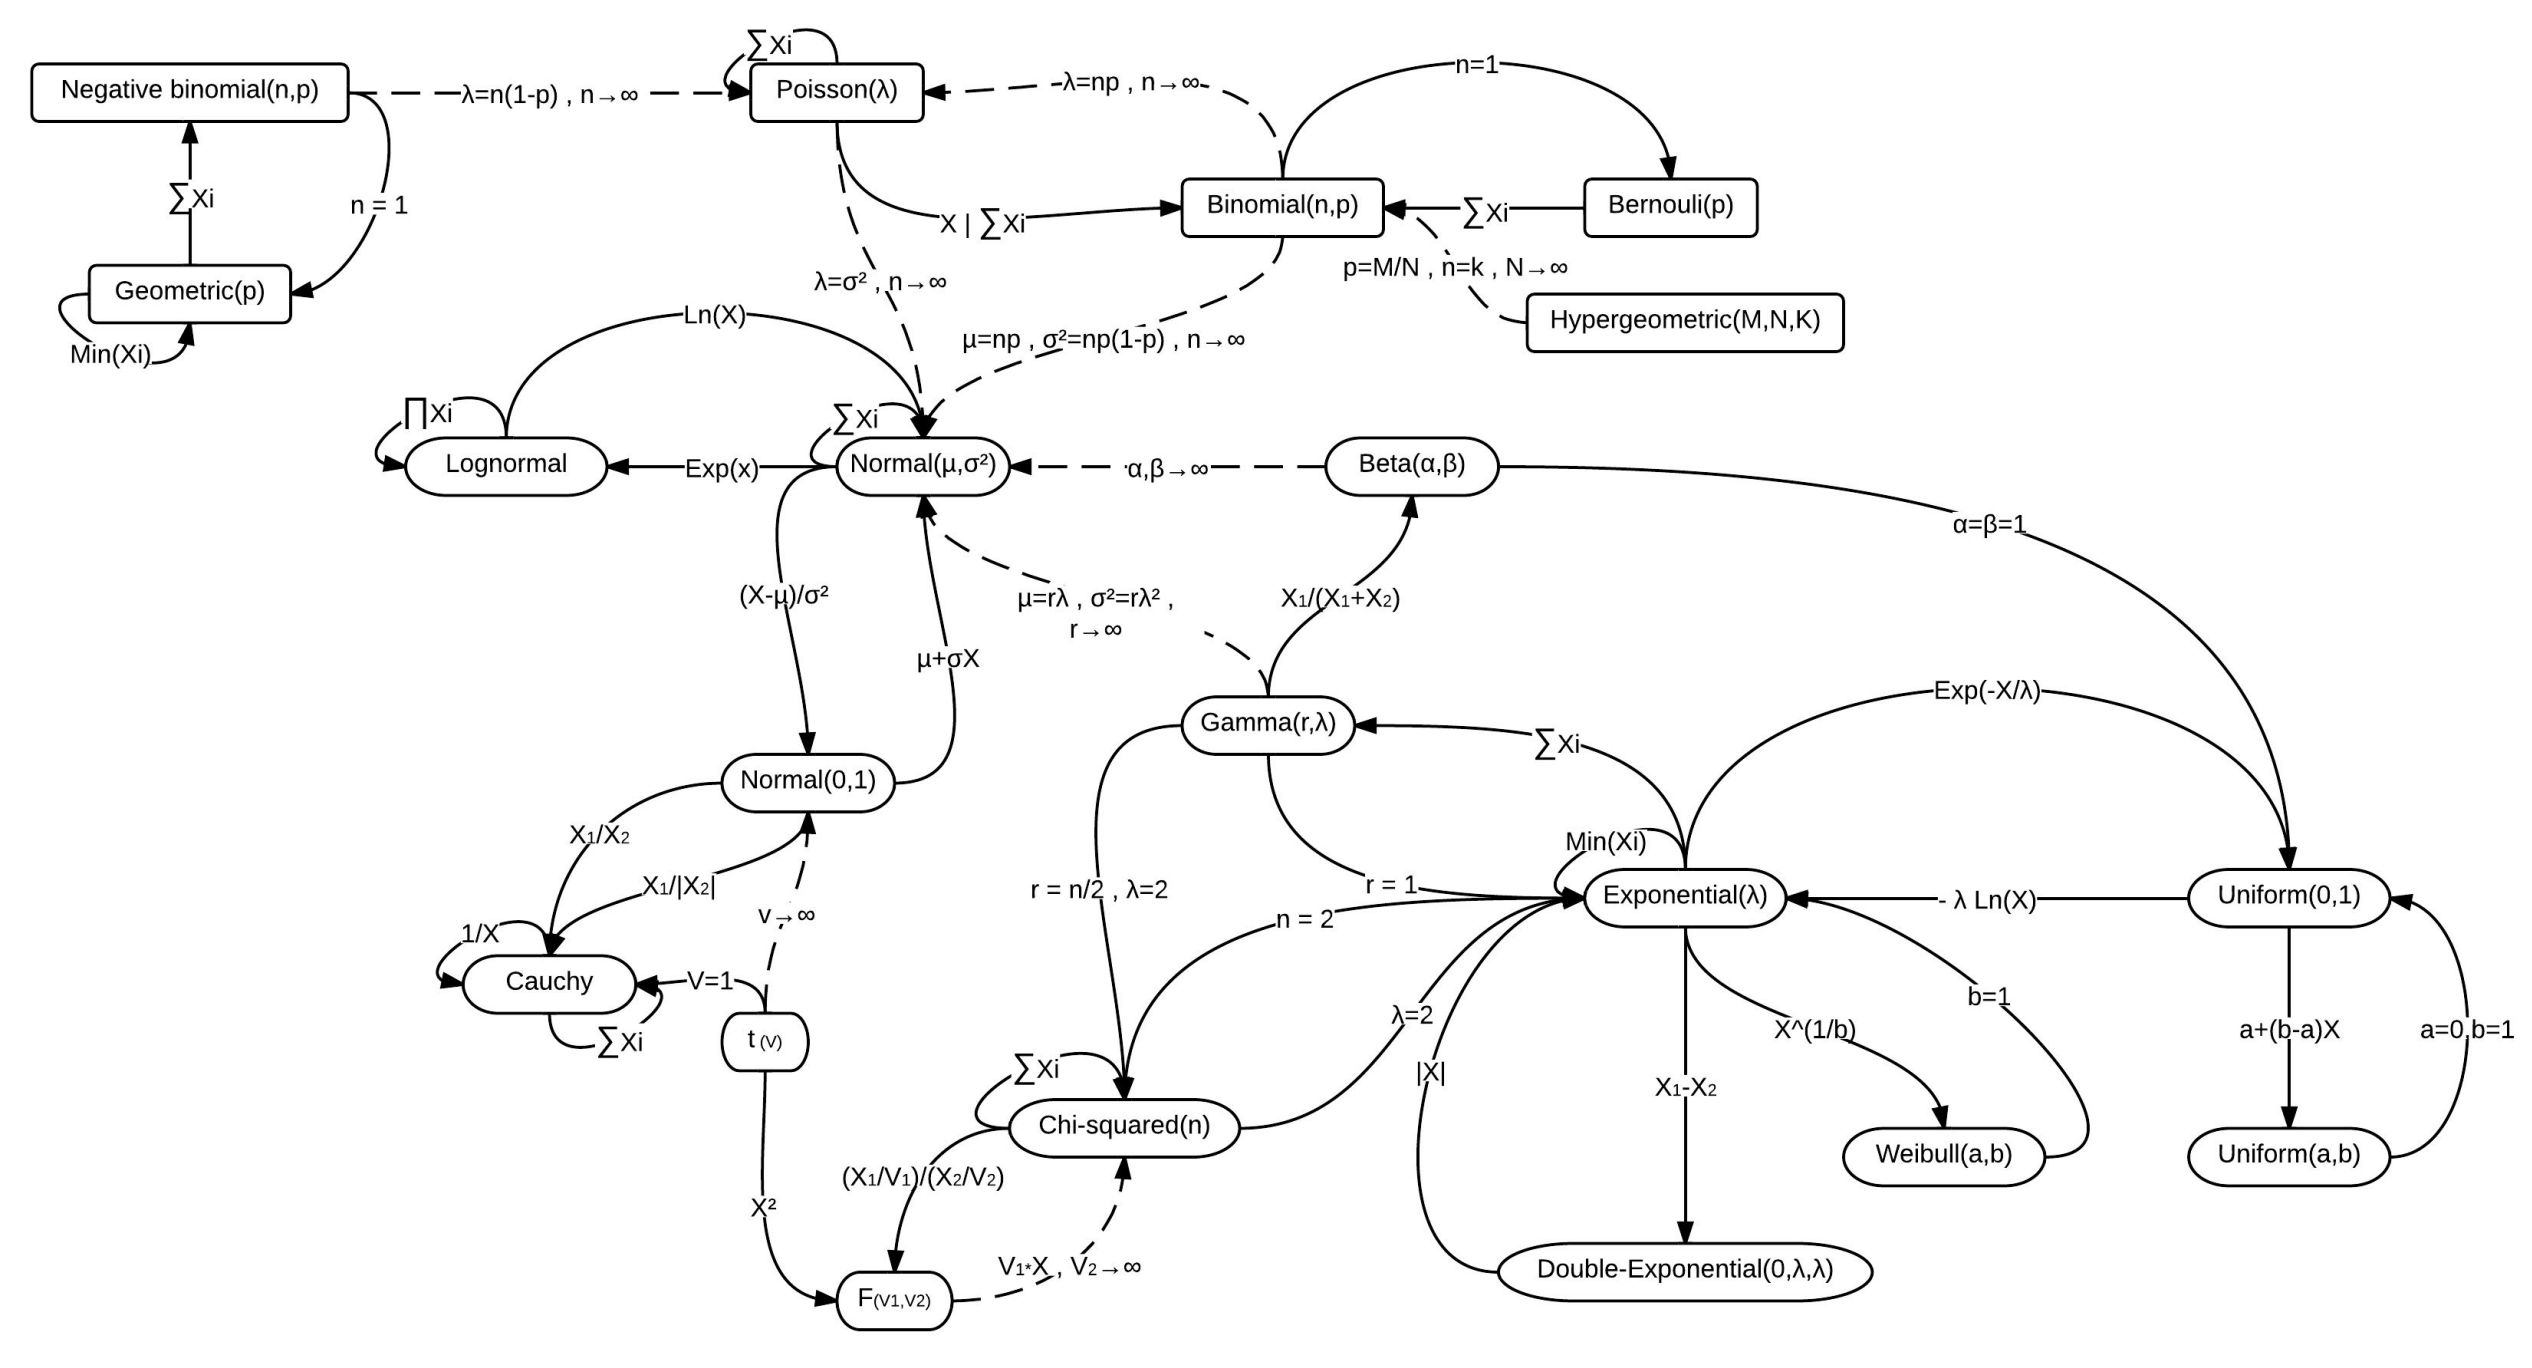
\includegraphics[scale=0.35]{transformations.png}
\caption{Transformation Relationships Between Distributions}
\end{figure}

There are three main methods of transformation:
\begin{enumerate}[nosep, noitemsep]
\item Univariate Transform
\item Multivariate Transform
\item Probability Integral Transform
\end{enumerate}

\subsection{Univariate Transform}

This is a transformation for one variable. Suppose we have a random variable $X$ and we want to get the probability distribution of some function of $X$, we can do this. 

ie. We have $X \sim f_X(x)$ and we want to get $f_Y(y)$ where $Y=g(X)$.


To do this we have to make the assumption that $g(X)$ is a one-to-one/injective function, that is $y=g(x)$ has only one solution (passes the horizontal line test).

Making that assumption we can solve for the cdf of $Y$ like so: \begin{align*}
F_Y(y) & = P(Y \leq y) \\
& = P(g(X) \leq y) \\
& = \int_{ \{x|g(x) \leq y\} } f_X(x) dx \\
& = \int_{-\infty}^{g^{-1}(y)} f_X(x) dx
\end{align*}
\noteworthy{F_Y(y) = \int_{-\infty}^{g^{-1}(y)} f_X(x) dx}{Univariate Transform cdf}

%And taking the derivative with respect to $y$: \noteworthy{f_Y(y) = \deriv{}{y} F_Y(y) = f_X(g^{-1}(y)) \abs{\frac{g^{-1}(y)}{dy}}}{Univariate Transform pdf}



%\item The probability of a value greater than a given $x$ is the cdf: \noteworthy{F(x) = P(X \leq x) = \int_{-\infty}^{x} f(t) dt}{cdf of continuous random variable}


Then determine the pdf by taking the derivative with respect to $y$: \begin{align*}
f_Y(y) & = \deriv{}{y} F_Y(y) \\
& = \deriv{}{y} \int_{-\infty}^{g^{-1}(y)} f_X(x) dx \\
& = \sqbr{ f_X \br{ g^{-1}(y) } \deriv{}{y} g^{-1}(y) } - \cancelto{0}{\sqbr{ f(-\infty) \deriv{}{y} (-\infty) } } & \text{By Leibniz integral rule}  \\ 
& = f_X \br{ g^{-1}(y) } \abs{ \frac{g^{-1}(y)}{dy} } & \text{Absolute because } f_Y(y) \geq 0 
\end{align*}
\noteworthy{f_Y(y) = f_X \br{ g^{-1}(y) } \abs{ \frac{g^{-1}(y)}{dy}}}{Univariate Transform pdf}

\subsubsection*{Example}

Suppose we have a noiseless non-Inverting amplifier. It takes in a signal $x$ and outputs the signal $y=ax$. 

If $x$ comes from Gaussian noise source $X \sim N(\mu, \var)$, what is the distribution of the output signal $f_Y(y)$?

\ex

Recall we make the assumption that $y=g(x)$, which means $g^{-1}(y) = x$, so: $$g^{-1}(y) = x = \frac{y}{a}$$

Using (\ref{Univariate Transform pdf}), we know: \begin{align*}
f_Y(y) & = f_X \br{ g^{-1}(y) } \abs{ \frac{g^{-1}(y)}{dy}} \\
& = f_X \br{ \frac{y}{a} } \abs{ \frac{\frac{y}{a}}{dy}} \\
& = \frac{1}{a} f_X \br{ \frac{y}{a} }
\end{align*} Plugging in $f_X(x) = \frac{1}{\sqrt{2\pi\var}} e^{\frac{-(x-\mu)^2}{2\var}}$ and simplifying, you get this relation: \begin{align*}
f_Y(y) & = N(a\mu, a^2, \var)
\end{align*}

\ex 

Now suppose $Y=g(X)$ is not injective, so we can't assume $x=g^{-1}(x)$, then how would we get $f_Y(y)$ given $f_X(x)$? Well, we could directly evaluate the following:

$$ f_Y(y) = \deriv{}{y}{} \br{ \int_{\{x|g(x) \leq y\}} f_X(x) dx }$$

But this is hard because we don't know what $\{x|g(x) \leq y\}$ is. So if $g(x)$ is not injective, then we can denote the $n$ roots of $y=g(x)$ by $\{X_i\}^n_{i=1}$. Then use the following, where $x_i = x_i(y)$:\noteworthy{f_Y(y) = \sum_{i=1}^n f_X(x_i) \abs{ \deriv{x_i}{y} }}{Univariate transformation relation}
% =  \sum_{i=1}^n f_X(x_i) \abs{ \deriv{y}{x_i}}^{-1}

\subsubsection*{Example}

A non-inverting amplifier takes an input signal $x$ and outputs the signal $y=ax^2$.

If $x$ comes from Gaussian noise $X \sim N(\mu, \var)$, what is the distribution of output signal $f_Y(y)$?

\ex

First determine the routes of $y=g(x) = ax^2$. \begin{align*}
 x_1  = \sqrt{\frac{y}{a}} & & \deriv{x_1}{y} = \frac{1}{2y} \sqrt{\frac{y}{a}} \\
 x_2  = -\sqrt{\frac{y}{a}} & & \deriv{x_2}{y} = -\frac{1}{2y} \sqrt{\frac{y}{a}}
\end{align*}

Now using (\ref{Univariate transformation relation}):\begin{align*}
f_Y(y) & = \sum_{i=1}^n f_X(x_i) \abs{ \deriv{x_i}{y} } \\
& =  f_X(x_1) \abs{ \deriv{x_1}{y} } + f_X(x_2) \abs{ \deriv{x_2}{y} } \\
& =  f_X\br{\sqrt{\frac{y}{a}}} \sqbr{ \frac{1}{2y} \sqrt{\frac{y}{a}} } + f_X\br{-\sqrt{\frac{y}{a}}} \sqbr{\frac{1}{2y} \sqrt{\frac{y}{a}} } \\
& = \frac{1}{2\sqrt{ya}} \sqbr{ f_X \br{\sqrt{\frac{y}{a}}} + f_X \br{-\sqrt{\frac{y}{a}}} }
\end{align*}

\ex




\subsection{Multivariate Transform}

Now given $V=g(X,Y)$, $h(X,Y)$, and $f_{XY}(x,y)$, we're going to learn how to get the joint pdf $f_{VW}(v,w)$.

Theoretically we could do something like: $$ f_{VW}(v,w) = \deriv{}{v} \deriv{}{w} \iint\limits_{\{(x,y)\ |\ g(x,y) \leq v,\ h(x,y)\leq w \}} f_{XY}(x,y)dxdy $$

But that's just ridiculous. It's impossible to visualize and begin defining event space here, so let's look at how to evaluate $f_{VW}(v,w)$ without needing explicit evaluation of multivariate integral limits:
\noteworthy{f_{VM}(v,w) = \sum_{i=1}^n f_{XY}(x_i, y_i) \abs{ \jac_i } \ \ \ \  \text{where} \ \abs{ \jac_i } = \abs{ \deriv{\phi_i}{v_i}  \deriv{\psi_i}{w_i} - \deriv{\phi_i}{w_i}  \deriv{\psi_i}{v_i} }}{Multivariate transformation relation}
Here the inverse-mappings of $(v,w)$ are given by $\{x_i = \psi_i(v,w),\ y_i=\phi_i(v,w)\}_{i=1}^n$, and $\abs{\jac}$ is the magnitude of the \textit{Jacobian}, which is equal to $A(\mathbb{R})/A(\mathbb{N})$.

\subsubsection*{Example}
$V = g(X,Y) = \sqrt{X^2 + Y^2}$ and $W = h(X,Y) = Y/X$.  

If $X\sim N(0, \var)$ and $Y\sim N(0,\var)$ are independent distributions, evaluate (a) $f_{VW}(v,w)$, and (b) show $f_{VW}(v,w)$ is independent. 

\ex

Solving the system: \begin{align*}
V  & = \sqrt{X^2 + Y^2} \\
W  & = Y/X 
\end{align*}
We get solution 1: \begin{align*}
x_1 = \phi_1(V,W)  & = \frac{V}{\sqrt{1 + W^2}} \\
y_1 = \psi_1(V,W)  & = \frac{WV}{\sqrt{1 + W^2}} 
\end{align*}
And solution 2:
\begin{align*}
x_2 = \phi_2(V,W) & = \frac{-V}{\sqrt{1 + W^2}} \\
y_2 = \psi_2(V,W) & = \frac{-WV}{\sqrt{1 + W^2}} 
\end{align*}

\begin{align*}
\abs{ \jac_1 } 
& = \abs{ \deriv{\phi_1}{v}  \deriv{\psi_1}{w} - \deriv{\phi_1}{w}  \deriv{\psi_1}{v} }  \\
& = \abs{ \deriv{}{v}\br{\frac{V}{\sqrt{1 + W^2}}}   \deriv{}{w}\br{\frac{WV}{\sqrt{1 + W^2}} } - \deriv{}{w}\br{\frac{V}{\sqrt{1 + W^2}}}  \deriv{}{v}\br{\frac{WV}{\sqrt{1 + W^2}} } }  \\
& = \abs{ \br{\frac{1}{\sqrt{1 + W^2}}}  \br{\frac{V}{(1 + W^2)^{3/2}} } - \br{\frac{-WV}{(1 + W^2)^{3/2}} } \br{\frac{W}{\sqrt{1 + W^2}} } }  \\
\end{align*} 

??? In his notes in \texttt{Lecture07hw.pdf} page 3, he says:  $$
\deriv{y_1}{v} = \deriv{}{v} \br{\frac{wv}{1+w^2}} = \frac{w}{1+w^2} = 0?
$$

\ex
\subsubsection*{Example}

Let $X \sim N(\mu_x, \var_x)$, $Y \sim N(\mu_y, \var_y)$ be the random variables associated with two independent sensors that provide an estimate of the position of a target.

A non-symmetric differential amplifier merges the signals, producing an estimate of the target's position. The noise of the estimate is given by $Z = aX-Y$ with $a \geq 0$. \begin{enumerate}[(a)]
\item Compute the pdf of $Z$
\item Evaluate $\mu_z$ and $\var_z$ using $f_Z(z)$
\item What is the optimal $a$ for zero average noise? What's the noise variance of this $a$?
\end{enumerate}

\ex

\begin{enumerate}[(a)]
\item 
\end{enumerate}

\ex

\subsection{Probability Integral Transform}

You can use this to test if your dataset $\set{x_i}_{i=1}^n$ resulted from a certain distribution $f_X(x)$. %You can use the chi-squared ($\mathcal{X}^2$) test to evaluate if your set is consistent with a uniform distribution. 

Given a cdf $F_X(x)$ then the random variable $Y=F_X(X)$ has a uniform distribution. \begin{align*}
F_Y(y) & = P(Y \leq y) \\
& = P(F_X(X) \leq y) \\
& = P(X \leq F_X^{-1}(y)) \\
& = F_X(F^{-1}_X(y)) \\
& = y
\end{align*}

Given a continuous random variable $Y = F_X(X)$, you can use the \textit{probability integral transform}, you cannot with discrete random variable samples. \noteworthy{F_X(X) \sim \text{Unif}(0,1)}{Probability Integral Transform}






\section{Generating Distributions}

We can use computers to generate random numbers with a specified probability density. We do this to model real world parameters that vary with these probabilities.

Stochastic means that you don't actually know exactly what a parameter's value is, you know with a certain probability what its range is.

\subsection{Inverse Transform Algorithm}

\subsubsection{Discrete}

The inverse transform algorithm is useful for any discrete distribution. 
 Given a uniform random number generator, how can we simulate a discrete distribution $P_X(X=x_i)=p_i$?

\begin{enumerate}
\item Generate random variable $u \sim U(0,1)$
\item Set $x = \begin{cases}
x_1 & u \in [0,p_1] \\
x_2 & u \in (p_1, p_1 + p_2) \\
\vdots & \vdots \\
x_n & u \in (\sum_{i=1}^{n-1} p_i, 1]
\end{cases}$
\end{enumerate}

Let's say: $$x = \begin{cases}
1 & \text{20\% of the time} \\
2 & \text{10\% of the time} \\
3 & \text{70\% of the time} \\
\end{cases}$$

Then you generate a uniform and if it falls between $[0,20]$, you assign the value 1. If the uniform falls between $(20,30)$, you assign value 2. Then for $ \in (30, 70]$, you assign 3. You get the idea.

\subsubsection{Continuous}

In the case that the distribution you want, say $F_X(x)$ is continuous, then it'll look like this: $$F_X(x) = P(X \leq x) = p$$ It takes $x$ as an input and outputs $p$. If you take the inverse of that function so: $$x = F^{-1}_X(p)$$ Then the input will be $p$, which is actually uniform so we'll call it $u$, and given uniform inputs will provide outputs $x$ in the desired distribution.

\textbf{Note}: You cannot use the inverse transform method to generate a Gaussian because there's no good CDF to take the inverse of.

The opposite of this is that if you want to generate a uniform, then you generate samples of a distribution, then you feed those values into that distribution's CDF and you'll get out a uniform distribution.

\subsection{Polar Algorithm}

You can construct anything from this method, it's particularly useful for generating a Gaussian which we can't do with the inverse method. 

\begin{enumerate}
\item Generate $u_1 \sim U(0,1)$, and $u_2 \sim U(0,1)$
\item Set $d=-2\ln{u_1}$ and set $\theta=2\pi u_2$
\item Set $x=\sqrt{d} \cos \theta$ and $y=\sqrt{d}\sin\theta$
\end{enumerate}

And by doing this, $X\sim N(0,1)$ and $Y\sim N(0,1)$ are independent normal random variables.

To then construct a non-standard normal distribution, use the linear properties and set: $$Z = \sigma X + \mu \ \ \ \ \ \text{where } X \sim N(0,1)$$


\subsection{Compositional Method}

If it's challenging to create a distribution using the inverse transform method, you can try the compositional method. 

The idea here is to decompose your desired distribution $F_X(x)$ from a sum of weighted distributions $F_{X_i}$. This is good if it's easy to generate samples from the  $F_{X_i}$ distributions. $$F_X(x) = \sum_{i=1}^n p_i F_{X_i}(x) \ \ \ \ \ \text{where} \sum_{i=1}^n p_1 = 1 \ \ \ p_i \geq 0$$ Then we can use the compositional method to generate samples from $F_X(x)$ \begin{enumerate}
\item Generate random variable $I$ which has a discrete distribution $P(I=i)=p_i$, for $i=1,2,\dots,n$.
\item Generate random variable $Y_I$ with distribution $F_{X_I}$ 
\item Set $X = Y_I$
\end{enumerate}





\subsection{Acceptance-Rejection Method}

Propose value, see if it gets accepted. Often use exponential because it goes from [0,$\infty$] and looks like a symmetrical side of normal.

Sampling something constrained between values use uniform, sampling something that's positive use exponential, sampling something that uses entire real line use normal.








%$$\hat{F}_X(x) = P(X(\mathbf{Y}_i) \leq x)$$

%\ex

%\textbf{Does the inverse of $\mathbf{F_X(x)}$ exist?}

%\ex

%Set $y=F_X(x)$, $x=F^{-1}(y)$. For the inverse $F_X^{-1}(y)$ to exist, each element $y \in Y$ must correspond to exactly one element of $x \in support \set{F_X(x)}$ -- this means for all $x$ where $F_X(x) > 0$.

%Since $F_X(x) = \sum_{x_i \leq x} P_X(x = x_i) u(x=x_i)$

%...

%Each element of $y \in Y$ corresponds to an unaccountably infinite elements in an interval on the real line. $F_x^{-1}(x)$ ...


%\textbf{Construct a method to generate samples from the random variable $X$ when $F_X(x) = Bernoulli(p)$.}

%... Proving, for instance on an exam always involves the same method $\hat{F_X}(x) = F_X(x)$. Know which method to apply. 

%In an inverse transform method, invert the probability distribution function, not the density function.

%For Gaussian random variable, you cannot use the inverse transform method.


%--------------------------------%

\section{Random Processes}

\subsection{Independent and Identically Distributed (IID)}

With IID distributions, each random variable has the same distribution (possible outcome) and all outcomes are mutually independent.

A random process is IID if:\begin{enumerate}
\item It has no memory, so past results tell us nothing about future results
$$P(X[k] = x_k | X[1], \dots, X[k-1]) = P(X[k] = x_k) = f_{X_k}(x_k;k)$$
\item Identical/time-invariant distribution
$$P(X[k] = x_k) = f_{X_k}(x_k;k) = f(x_k)$$
\end{enumerate}

And IID process is actually a special case of a Markov chain, which we get to in section \ref{Markov Section}.

\subsection{Markov Chain} \label{Markov Section}

Most sources have some sort of correlated random process, and are not pure IID. Markov Chains are a very important type of dependent stochastic process, and almost all engineering, economics, and social sciences model is Markov. 

Whereas IID processes have no memory: \noteworthy{P(X[k]\ |\ X[k-1], X[k-1], \dots) = P(X[k])}{IID Process}

Markov chains do have some sort of memory: \noteworthy{P(X[k]\ |\ X[k-1], X[k-1], \dots) = P(X[k]\ |\ X[k-1]) \forall k}{First-order Markov chain}

They are characterized by three ingredients: \begin{enumerate}
\item \textbf{State space} -- $S = \set{x_1, \dots, x_m}$
\item \textbf{Initial state distribution} -- $\pi[0]$ (M dimensional column vector)

$\pi[0] = [P(X[0] = x_1), P(X[0] = x_2), \dots, P(X[0] = x_M)]'$

Clearly, $\pi ' [0] \mathbf{1} = 1$  -- ??? WHAT THE FUCK DOES THIS MEAN

\item Transition probability matrix: $A = (a_{ij})$ which is an $M \times M$ matrix $$\sum_{j=1}^M a_{ij} = 1 \implies A_{M\times M} \mathbf{1}_{M\times 1} = \mathbf{1}_{M \times 1}$$

In this matrix $A$, each row sums to 1, and all elements are non-negative.

\end{enumerate}

\subsubsection*{Example}
Consider a two-state Markov chain ($M=2$) with $\pi[0] = [0.3, 0.7]'$

\begin{figure}[ht!]

\begin{tabular}{cc}
$A = \begin{bmatrix}
0.8 & 0.2 \\
0.6 & 0.4 \\
\end{bmatrix}$ & 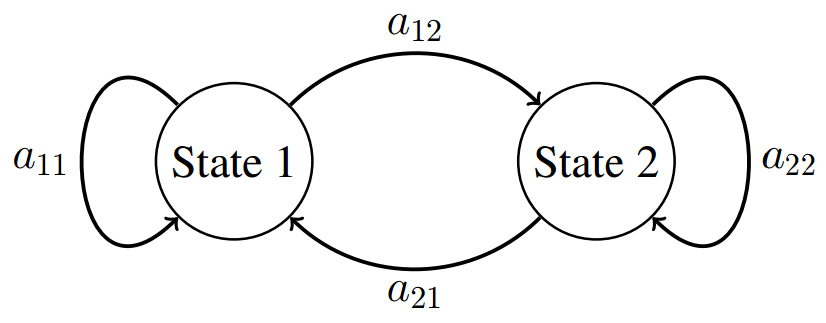
\includegraphics[scale=0.5]{m1.png}
\end{tabular}

\end{figure}

\textbf{Remarks about this Markov chain} \begin{itemize}
\item $a_{ij} = P(X[x+1] = j\ |\ X[k]=i)$, denotes the transition probability from state $i$ to state $j$. $a_{ii}$ denotes the probability of remaining in state $i$.

\item $A$ always has one eigenvalue at $\lambda = 1$ corresponding to eigenvector $\mathbf{1}$ because $A \mathbf{1} = \mathbf{1}$
\item $A^k$ is always a stochastic matrix for any integer  $k > 0$ --- meaning this is a first-order \textit{homogeneous} Markov Chain because $A$ is not a function of time (???)
\item Markov property means that there is \textit{conditional independence}, in that given $X[k]$, $X[k+1]$ is independent of the past (???)
\end{itemize}

\subsubsection{Stationary Distribution}

How can we compute the \textbf{steady-state probability} (stationary distribution), $\pi[\infty]$ of a Markov chain?

If we calculate $\pi[\infty]$ then we can model any source by a Markov chain, estimate the transition probabilities, and compute how much info it has. 

We do this using the \textbf{Chapman-Kolomorov Equation}. Given $\pi[0]$ and $A$, the state probability vector at time $k$ is given by: $$\pi[k] = [P(X[k] = x_1), \dots, P(X[k] = x_M)]'$$ 
This can be computed by: \noteworthy{\pi[k+1] = A'\pi[k] = (A')^{k+1}\pi[0]}{Chapman-Kolmogorov Equation}



\newpage
\bibliography{references}
\bibliographystyle{apacite} 
\pagebreak


% -------- APPENDIX -------- %
\appendix
\onehalfspacing
\chapter*{Appendix}
\addcontentsline{toc}{section}{Appendix}
\renewcommand{\thesubsection}{\Alph{subsection}}

\subsection{Tutorial 1 (Lena)}

\subsubsection*{Example 1}

Where $A$ and $B$ are events and:

$$P(A) = \frac{3}{4};\ P(B)=\frac{1}{3}$$

Show:

$$\frac{1}{12} \leq P(A \cap B) \leq \frac{1}{3}$$


---

First thing to note is that the intersection cannot be larger than the smallest $P$, so this is the upper bound: $$P(A \cap B) \leq \frac{1}{3}$$

From the inclusion-exclusion, $P(A \cap B) = P(A) + P(B) - P(A \cup B)$. Since $0 \leq P(A \cup B) \leq 1$, then the minimum bound is where $P(A \cup B) = 1$ and: $$P(A \cap B) \geq P(A) + P(B) - 1 = \frac{1}{3} + \frac{3}{4} - 1 = \frac{1}{12}$$


\subsubsection*{Example 2}

Prove: $$P(\cup_{n=1}^k A_n) \leq \sum_{n=1}^{n} P(A_n)$$

---

\begin{proof}[Proof]

Consider the base case, $n=2$. By the inclusion-exclusion principle:
$$P(\cup_{i=1}^2 A_i) = P(A_1 \cup A_2) = P(A_1) + P(A_2) - P(A_1 \cap A_2)$$
Since $P(A_1 \cap A_2) \geq 0$, then  $$P(\cup_{i=1}^2 A_i) \leq P(A_1) + P(A_2) 
 = \sum_{i=1}^{2} P(A_i)$$
Induction hypothesis, for $k \in \mathbb{N}$: $$P(\cup_{i=1}^k A_i) \leq \sum_{i=1}^{k} P(A_i)$$
For $k+1$, by the inclusion-exclusion principle:


$$P ( \cup_{i=1}^{k+1} A_i ) = P(\cup^k_{i=1} A_i \cup A_{k+i}) \leq P(\cup_{i=1}^k A_i) + P(A_{k+1})$$ $$ \leq \sum_{i=1}^k P(A_i) + P(A_{k+1}) = \sum_{i=1}^{k+1} P(A_i) $$
  
\end{proof}

\subsubsection*{Problem 1.1}

\begin{enumerate}[(a)]

\item $P(\overline{B}) = 1 - P(B) = \frac{2}{3}$

\item $P(A \cup \overline{B}) = P(A) + P(\overline{B}) - P(A \cap \overline{B}) \rightarrow P(A) = P(A \cap B) + P(A \cap \overline{B})$

\item $P(\overline{A} \cap B) \rightarrow P(B) = P(A \cap B) + P(\overline{B} \cap \overline{A})$

\item $P(\overline{A} \cup B) = P(\overline{A}) + P(B) - P(\overline{A} \cap B)$

\end{enumerate}


\subsubsection*{Problem 1.3}

$A$, $B$, and $C$ are mutually exclusive, so they are not independent. Additionally, they have no intersections.


\begin{enumerate}[(a)]

\item $P(A \cup B \cup C) = P(A) + P(B) + P(C)$

\item $P(\overline{A} \cup \overline{B}) = 1$

\item $P(\overline{A} \cap \overline{B}) = 1 - P(A) - P(B)$ 


\end{enumerate}

\subsubsection*{1.4}

\begin{enumerate}[(a)]

\item $P(A_{good}) = \frac{3}{5}$

\item $$P(B_{good} | A_{good}) = \frac{P(B_{good} \cap A_{good})}{P(A_{good})} = \frac{\frac{{3 \choose 2}}{{5 \choose 2}}}{\frac{3}{5}} = \frac{\frac{3}{10}}{\frac{3}{5}} = \frac{1}{2}$$

$$P(B_{good} | A_{bad}) = \frac{P(B_{good} \cap A_{bad})}{P(A_{bad})} = \frac{1}{2} \times \frac{\frac{{3 \choose 1}{2 \choose 1}}{{5 \choose 2}}}{1 - \frac{3}{5}} = \frac{1}{2} \times \frac{\frac{3}{5}}{1 - \frac{3}{5}} = \frac{3}{4}$$

Times by 1/2 because we only want the case, $B_{good}$ and $A_{bad}$.

\item 

\item $$P(A_{good} \cap B_{good}) = \frac{{3 \choose 2}}{{5 \choose 2}}$$

\item $$P(B_{good}) = P(B_{good} \cap A_{good}) + P(B_{good} \cap A_{bad}) = \frac{{3 \choose 2}}{{5 \choose 2}} +  \frac{\frac{1}{2} \times {3 \choose 1}{2 \choose 1}}{{5 \choose 2}}$$

\end{enumerate}

\subsubsection*{Problem 1.5}

\begin{enumerate}[(a)]

\item $$P(\{ balls\ are\ red\}) = \frac{{7 \choose 2}}{{15 \choose 2}}$$

\item $$P(\{ both\ same\ colour\}) = \frac{1}{{15 \choose 2}}$$

\item $$P(\{ 2nd\ is\ green\})  = P(G_2 | G_1)P(G_1) + P(G_2|B_1)P(B_1) + P(G_2|R_1)P(R_1)$$

$$\frac{4}{14} + \frac{5}{15} + \frac{5}{14} \times \frac{10}{15}$$

\end{enumerate}



\subsection{Tutorial 2 (Yang)}

\subsubsection*{1.9}

10 keys $\rightarrow$ 1 correct. No replacement.

Define $A_i = \{ $ $i$th attempt works $\}$

\begin{enumerate}[(a)]
\item $P(A_1) = \frac{1}{10}$
\item $P(A_2) = P(A_1^c \cap A_2) = P(A_2|A_1^c) P(A_1^c) = \frac{1}{9} \frac{9}{10} = \frac{1}{10}$

Alternatively, $P(A_2) = P(A_1 \cap A_2) + P(A_1^c \cap A_2)$ where $P(A_1 \cap A_2)$ because only 1 can be correct.

\item $P(A_i) = P(A_1^c \cap \dots \cap A_{i-1}^c \cap A_i) = P(A_i | A_1^c \cap \dots \cap A_{i-1}^c) \times P(A_{i-1}^c | A_{i-2}^c \cap \dots \cap A_{1}^c) \dots P(A_1^c) = 1/10$

\item 

\begin{table}[H]
\centering
\begin{tabular}{c|cccc}
\toprule
\# of attempts & 1 & 2 & 3 & $\dots$ 10 \\
\midrule
$p_i$ & 1/10 & 1/10 & 1/10 & $\dots$ 1/10 \\
\bottomrule
\end{tabular}
\end{table}

$$
E(x) = \sum_{i=1}^n x_i p_i = 1/10 + 2/10 + 3/10 + \dots + 10/10 = 55/10 = 5.5
$$



\end{enumerate}

\subsubsection*{1.10}


10 keys $\rightarrow$ 1 correct. Yes replacement.

Define $A_i = \{ $ $i$th attempt works $\}$

\begin{enumerate}[(a)]
\item $P(A_1) = \frac{1}{10}$
\item $P(A_2) = P(A_1^c \cap A_2) = P(A_2|A_1^c) P(A_1^c) = \frac{1}{10} \frac{9}{10} = \frac{9}{100}$


\item Probability that all attempts up to $i$ didn't work and that $i$ did. 

$P(A_i) = P(A_1^c \cap \dots \cap A_{i-1}^c \cap A_i) = (\frac{9}{10})^{i-1} \frac{1}{10}$

\item  $x$ = \# of first successful attempts, $p_i = P(X = x)$

\begin{table}[H]
\centering
\begin{tabular}{c|ccccc}
\toprule
$x_i$ & 1 & 2 & 3 & $\dots$ & $\infty$ \\
\midrule
$p_i$ & 1/10 & $(9/10)^1$ 1/10 & $(9/10)^2$ 1/10 & $\dots$ & \\
\bottomrule
\end{tabular}
\end{table}

$$
E(x) = \sum_{i=1}^n x_i p_i = \sum_{i=1}^{\infty} i \left(\frac{9}{10}\right)^{i-1} \frac{1}{10}
$$

If doing infinite sum, probably need to be a geometric series. Might also be telescoping sum, but most likely geometric series.

Geometric series: $\sum_{i=0}^{\infty} p^i = \frac{1}{1-p}$ where $|p|<1$.

Differentiate w.r.t p: $$\sum_{i=0}^{\infty} i p^{i-1} = \frac{1}{(1-p)^2} $$

 $$\sum_{i=1}^{\infty} i p^{i-1} = \frac{1}{(1-p)^2} $$

Multiply both sides by $(1-p)$:  $$\sum_{i=1}^{\infty} i p^{i-1} (1-p) = \frac{1}{1-p} $$

Since $p=9/10$: $$\frac{1}{1-p} = 10 $$

So he will likely grab it on the 10th try.


\end{enumerate}

\subsubsection*{1.11}

First some stuff to recall: 

 Sensitivity is that if the patient is sick, the test will be positive. Specificity is that if the patient is not sick, that the test will be negative.
 
Equation (0): $$P(A|B) = \frac{P(A \cap B)}{P(B)}$$ 

Equation (1): $$P(A \cap B) = P(A|B) P(B) = P(B|A) P(A)$$

Equation (2): $$P(A) = P(B|A) P(A) + P(B^c|A) P(A) $$

Equation (3): $$ P(B|A) +P(B^c|A) = 1 $$

Equation (4): 

Conditional independence, events $A_1$ and $A_2$ are independent on B: $$ P(A_1 \cap A_2 | B) = P(A_1 | B) P(A_2 |B) $$

General independence: $$P(A_1 \cap A_2) = P(A_1) P(A_2)$$

---

Given $E = \{$ patient is sick $\}$. $T_i = \{$ test result $i$ positive $\}$, $i=1,2,3,4,5$.

$T_i$ are conditionally independent given $E$ and $E^c$.

Known: $P(E)$, $P(T_i|E)$, $P(T_i^c|E^c)$

$$P(T_i^c|E) = 1-P(T_i|E) \rightarrow $$

\begin{enumerate}[(a)]

\item $P(E|I_n)$, $I_n=T_1 \cap T2 \cap \dots \cap T_5$. From $\frac{(1)}{(2)}$.

$$P(E|I_n) = \frac{P(E \cap I_n)}{P(I_n)}  \frac{P(I_n|E) P(E)}{P(I_n \cap E) + P(I_n \cap E^c}$$ 

Look at notes online...

$$ = \frac{P(T_1|E) \times \dots \times P(T_n|E) \times P(E)}{P(T_1|E) \dots } $$

\item Sequential updates. $I_{k+1} = T_1 \cap T2 \cap ... T_k \cap T_{k+1}$.

$$P(E|I_{k+1}) = \frac{P(E \cap I_{k+1})}{P(I_{k+1})}$$

\textbf{Numerator}, from (1): $$ P(E \cap I_{k+1}) = P(I_{k+1} \cap E) = P(I_{k+1}|E)P(E)$$ $$= P(T_1 \cap T2 \cap ... T_k \cap T_{k+1} | E)P(E) $$
$$= P(I_k \cap T_{k+1} | E)P(E) $$
Because independent, from formula (4): $$= P(I_k | E)P(T_{k+1}|E)P(E) $$

Unite $P(I_k|E)P(E) = P(I_k \cap E)$ from (1): $$ = P(I_k \cap E) P(T_{k+1}|E)$$ $$ = P(E | I_k) P(I_k) P(T_{k+1}|E)$$
Call this result ($\star$).

\textbf{Denominator}: $$P(I_{k+1}) = P(I_{k+1} \cap E) + P(I_{k+1} \cap E^c$$

Conditioning on $E^c$:
$$ P(I_{k+1} \cap E^c) = P(I_{k+1}|E^c) P(E^c)$$
$$ = P(I_k \cap T_{k+1} | E^c) P(E^c) $$
$$ = P(I_k | E^c) P(T_{k+1}|E^c) P(E^c)$$
$$ = P(I_k \cap E^c) P(T_{k+1}|E^c)$$
$$ = P(E^c|I_k) P(T_{k+1}|E^c) P(I_k)$$
Call this result ($ \star \star $).

Putting this all together: $$P(E|I_{k+1}) = \frac{(\star)}{(\star) + (\star \star)} = \frac{P(E | I_k) P(I_k) P(T_{k+1}|E)}{P(E | I_k) P(I_k) P(T_{k+1}|E) + P(E^c|I_k) P(T_{k+1}|E^c) P(I_k)}$$

Canceling out $P(I_k)$, we get our update formula: $$P(E|I_{k+1}) = \frac{(\star)}{(\star star)} = \frac{P(E | I_k) P(T_{k+1}|E)}{P(E | I_k) P(T_{k+1}|E) + P(E^c|I_k) P(T_{k+1}|E^c) }$$

\item 

$P(E) = 0.005$, $P(T_i |E ) = 0.99$, $P(T_i^c | E^c) = 0.99$.

Since this is our first test, we use just $P(E)$ as our history:

Test 1 negative: $$  P(E|T_1^c) = \frac{P(E) P(T_1^c|E)}{P(E) P(T_1^c|E) + P(E^c) P(T_1^c |E^c)} = \frac{0.005 \times 0.01}{0.005 \times 0.01 + (1-0.005) \times 0.99} = 5.1(10)^{-5}$$

Test 2 positive, so no complement over $T_2$. And $I_k = T_1^c$: $$ P(E|T_1^c \cap T_2) =\frac{P(E|T_1^c) P(T_2|E)}{P(E|T_1^c) P(T_2|E) + P(E^c|T_1^c) P(T_2|E^c)}$$ $$= \frac{5.1(10)^{-5} \times 0.99}{5.1(10)^{-5} \times 0.99 + (1-5.1(10)^{-5}) \times 0.01} = 0.005$$

Best guess is still just the incidence of disease since the two tests contradict each other and neither is weighted more than the other.

Test 3 positive: $$P(E|T_1^c \cap T_2 \cap T_3) =\frac{P(E|T_1^c \cap T_2) P(T_3|E)}{P(E|T_1^c \cap T_2) P(T_3|E) + P(E^c|T_1^c \cap T_2) P(T_3|E^c)} $$ $$ = \frac{0.005 \times 0.99}{0.005 \times 0.99 + (1-0.005) \times 0.01} = 0.332 $$

Test 4 positive: $$P(E|T_1^c \cap T_2 \cap T_3 \cap T_4) $$ $$= \frac{0.332 \times 0.99}{0.332 \times 0.99 + (1-0.332) \times 0.01} = 0.9301 $$

Test 5 positive: $$P(E|T_1^c \cap T_2 \cap T_3 \cap T_4 \cap T_5) = 0.9997 $$

\subsubsection*{Aside}

Difference between events and probabilities.

Events: $P(A \cup B)$ works, $P(A+B)$ doesn't.

Probabilities: $P(A) + P(B)$ works, $P(A) \cup P(B)$ doesn't. Probabilities are numbers, events aren't.

\end{enumerate}

\subsection{Tutorial 3 (Lena)}

\subsubsection{Random Variables Revisited}

Usually notated with an upper case letter, say $X$.  The thing that differentiates it from an unknown $x$ is that it can change on the fly.

It is based on the probability density function, PDF, $f_X(x)$, where the subscript is the random variable and the input is the x-axis.

Densities can take values above 1, it is not a probability, it is a measure of relative frequency. We only use this when we're plotting or integrating. Usually it's a pain otherwise.

The cumulative distribution function, CDF, $F_X(x)$ is the probability that our input variable $x \leq X$. Cumulative because it sums PDF. $$F_X(x) = P(X \leq x) = \int_{-\infty}^{\infty} f_x(t) dt$$

The \textbf{quantile}, $q$, is such a value of $x$ that is the inverse of the CDF. Where $p$ is the area under the $f_X(x)$ curve below $x=q$. $$P(X \leq q) = p$$

1st quantile median. $$P(X \leq q) = 0.25$$ $$P(X \leq q) = 0.5 = F_x(q)$$

Properties of CDFs and PDFs:

\begin{enumerate}
\item PDF \begin{enumerate}
\item $f_X(x) \geq 0$
\item if $a \leq x \leq B$, then $f_X(x) = 0$ for $x \in (-\infty, a] \cup [B, \infty)$
\item $\int_{-\infty}^{\infty} f_X(x) = 1$
\end{enumerate}
\item CDF \begin{enumerate}
\item $ 0 \leq F_X(x) \leq 1 $
\item if $a \leq x \leq B$,then \\ $F_X(B) = 1 = P(X \leq B)$ and $F_X(a) = 0 = P(X \leq a)$
\item $F_X(x)$ is non-decreasing in $x$
\end{enumerate}
\end{enumerate}

\subsubsection{Uniform Distribution}

When the PDF is plotted, looks like a rectangle.

$$ f_X(x) = \frac{1}{b-a},\ a \leq x \leq b $$
$$ F_X(x) = \frac{x-a}{b-a},\ a \leq x \leq b$$

Since the probability is the same everywhere, if you integrate you'll see that the expected value is just in the middle.
$$E(X) = \frac{a+b}{2}$$
$$Var(X) = E(X^2) - E(X)^2 = \frac{(b-a)^2}{12}$$

\subsubsection{Exponential Distribution}

When the PDF is plotted, it looks like a typical delay.

Usually used to model time between events. There is only one parameter $\lambda$, which is the rate per item of time or per space. $X$ is then measured in units of whatever $\lambda$ is.

$X \sim Exp(\lambda)$

$$f_X(x) = \lambda e^{-\lambda x}, x \geq 0$$
$$F_X(x) = 1-e^{-\lambda x}, x \geq 0$$
$$E(x) = \frac{1}{\lambda}$$


\subsubsection*{Example}

$\lambda = 3/day$. $X = $ time until next call. So $X \sim Exp(3)$.

What is the probability that the next call is within 5-6 hours? $$P(5\ hours \leq X \leq 6\ hours)$$ $$P(5/24\ days \leq X \leq 6/24\ days)$$
$$ = \int_{5/24}^{6/24} 3e^{-3x} dx = F(6/24) - F(5/24) = (1-e^{-3(6/24)}) - (1-e^{-3(5/24)}) $$

What is the median time until the call? This means when 50\% of the time is below and 50\% of the time is above. $$F_X(m) = 0.5 = 1-e^{-3m} \rightarrow \text{solve for}\ m$$

Expected time for a call is $\frac{1}{\lambda}$. Variance is $\left( 1/\frac{3}{24} \right)^2$ 

\subsubsection{Normal Distribution}

$f_X(x)$ looks like a bell-curve, symmetric around $\mu$. Parameters are $\mu$, the mean, and $\sigma^2$, the variance.

$$ f_X(x) = \frac{1}{\sqrt{2 \pi} \sigma} e^{\frac{-(t-\mu)^2}{2 \sigma^2}}$$ $$F_X(x) = \dots = \Phi(x)$$ 

We can't evaluate the CDF in closed-form integration.
$$E(X) = \mu$$ $$Var(X) = \sigma^2$$

Specific case we'll often see is \textbf{standard normal}, $Z$. At which $Z \sim N(0,1),\ \mu=0$ and $\sigma^2=1$.
$$ X \sim \mu(\mu, \var)$$ $$ Z = \frac{X-\mu}{\sigma}$$
$$\Phi(-c) = 1-\Phi(c)$$
$$P(|Z|\leq c) = P(-c \leq Z \leq c) = \Phi(c) - \Phi(-c) = 2\Phi(c) -1 $$ 

Since we can't integrate in closed-form, we'll use $R$ functions.

CDF can be found using $\Phi(c) = \texttt{pnorm(c)}$.
$$\Phi(2) = P(Z \leq 2) = 0.9772$$ This is the area under the curve until the point $x=2$.

Note: Symmetry means the median is the same as the mean.

For quantities, $\Phi(c) = 0.75$, where $c=\texttt{qnorm(0.75)}=0.674$. This means that the area under the curve at the point $x=0.674$ is $75\%$ of the area under the curve.

\subsubsection*{Problem B.5}

$Z \sim N(0,1)$, $\Phi(1)=0.3413$.

\begin{enumerate}
\item \begin{enumerate}
\item $P(-1 < Z < 1)$ 

$$P(-1 < Z < 1) = P(Z < 1) - P(Z < -1) = \Phi(1) - \Phi(-1) $$ $$ = \Phi(1) - (1-\Phi(1)) = 2\Phi(1) - 1 = 0.6826$$
\item $P(Z > 1)$
$$P(Z > 1) = 1-P(Z \leq 1) = 1-\Phi(1) = 0.1587$$
\item $P(Z < -1)$
$$ P(Z < -1) = \text{same as above by symmetry}$$

\end{enumerate}
\item \begin{enumerate} 
\item  Note there are typos here, the $P(Z<c)$ should say $c_1$ and $c_2$ respectively. $c_1$ is larger.

$$\Phi(c_2) = 0.8,\ c_2 = \texttt{qnorm(0.8)} = 0.84$$
$$P(|Z|<c_1) = 2\Phi(c_1) - 1 = 0.8$$
$$\Phi(c_1) = 1.8/2 = 0.9$$
$$c_1 = \texttt{qnorm(0.9)} = 1.28$$


\end{enumerate}
\end{enumerate}

---

Non-standard normal. $$ X \sim N(\mu, \var)$$

$X = \mu + \sigma Z$, where $Z \sim N(0,1)$

$$P(X \leq c) = P(\frac{x-\mu}{\sigma} \leq \frac{c-\mu}{\sigma} ) = P(Z \leq \frac{c-\mu}{\sigma}) = \Phi(\frac{c-\mu}{\sigma})$$

Properties $X_1 \sim N(\mu_1, \var_1)$ and $X_2 \sim N(\mu_2, \var_2) $

\begin{itemize}
\item $X_1 \pm X_2$, $ \sim N(\mu \pm \mu_2, \var_1 + \var_2)$
\item $aX_1 \pm BX_2$, $ \sim N(a\mu \pm B\mu_2, a^2\var_1 + B^2\var_2)$

Important distinction $$Var(aX_1) = a^2 Var(X_1) = a^2 \var$$ $$Var(X_1 + X_2) = Var(X_1) + Var(X_2) = \var_1 + \var_2 $$
\end{itemize}

\subsubsection*{Example}

Distribution of grades is normal mean 75 and standard deviation is 10. Define $X$ as the test score of the student.

\begin{enumerate}
\item What is the probability that a random student passes? $$X \sim N(75, 10^2) $$ $$ P( \frac{X-75}{10} \geq \frac{50-75}{10} $$ $$ P(Z \geq -2.5) $$ $$ 1- P(Z < -2.5) $$ $$ 1-\Phi(-2.5) = \texttt{1 - pnorm(-2.5)} = 0.993709 $$

\item What is the $P$ that the student scored higher than average but lower than 85?

$$ P(75 \leq X \leq 85) = P(\frac{75-\mu}{\sigma} \leq \frac{X-\mu}{\sigma} \leq \frac{85-\mu}{\sigma} ) $$
$$ = P(\frac{75-75}{10} \leq Z \leq \frac{85-75}{10}  $$ $$ = P(0 \leq Z \leq 1) = \Phi(1) - \Phi(0) = \texttt{pnorm(1) - 0.5} = 0.3413  $$

\end{enumerate}
\subsubsection*{Problem 3, Lecture 4}

A machine fills "10-pound bags" of concrete mix. The actual weight is normally distributed with standard deviation of $\sigma = 0.1$ lbs. The mean is set by operator. Let $X$ by the weight of the bag, where $$X \sim N(\mu, 0.1^2)$$

\begin{enumerate}
\item What $\mu$ do we need if at most 10\% of bags should be underfilled ($<10$lbs)?

$$ P(X < 10) \leq 0.10 $$
Standardize, subtract the mean.

$$P(\frac{X -\mu}{\sigma} < \frac{10-\mu}{\sigma}) = P(Z < \frac{10-\mu}{0.1}) \leq 0.1$$

Solve $\Phi(\frac{10-\mu}{0.1}) = 0.1$ 

$$\texttt{qnorm(0.1)} = -1.2316 = \frac{10-\mu}{0.1} \rightarrow \mu=10.128$$

If you increase $\mu$, you decrease the probability that the $X < 10\%$ because you reduce the area under the curve below 0.1.

So for $P(X < 10) \leq 0.1$, we need $\mu \geq 10.128$.

\item Now define $\sigma=0.1 \mu$. Hence we have $X \sim N(\mu, 0.1^2\var)$. Same question as above.

Standardize again: $$ P(X < 10) = P \left( \frac{X -\mu}{\sigma} < \frac{10-\mu}{\sigma} \right) = P \left(Z < \frac{10-\mu}{0.1 \mu} \right) = \Phi \left( \frac{10-\mu}{0.1 \mu} \right)$$
$$ \frac{10-\mu}{0.1\mu} = -1.216 (???) \rightarrow \mu \geq 11.47 $$



\end{enumerate}

\subsubsection{Failure Rates}

Easy problems, just know the definitions of CDF and PDF. 

\subsubsection*{Example}

Lifetime of relationship has failure rate in years: $$\lambda(t) = \frac{1}{4} e^{-t}$$

\begin{enumerate}
\item Are relationships stronger or weaker over time?

Since the failure rate decreases over time, then the chance that the relationship breaks is shorter the longer the relationship is, so relationships get stronger over time.

\item Mike has just started to date Lindsey. What is the probability that their relationship survives 6-months. $X$ = duration of relationship.

$$F_X(x) = 1 - \exp{\int_0^x \lambda(t) dt}$$

$$ P(X > 0.5) = 1- P(X \leq 0.5) = 1 - F_X(0.5) = 1-(1-\exp(- \int_{0}^{0.5} \frac{1}{4} e^{-t} dt))$$ $$ = \exp(- \int_{0}^{0.5} \frac{1}{4} e^{-t} dt) = \exp(\frac{1}{4} e^{-0.5} - \frac{1}{4}) = 0.90631 $$ 

We solved this on the fly. Don't take it as gospel.

\item Find the median lifetime $F_X(m) = 0.5$.

$$1-\exp(- \int_{0}^{m} \lambda(t) dt) = 0.5$$
\end{enumerate}

\subsection{Midterm Review Session}

Let's take a look at the moment generating function for a binomial distribution, $$Y \sim Bin(n,p)$$.

You should know, the moment generating function is: $$M(t) = (1-p+pe^t)$$ 

To get the expected value, take: $$E(X) = M'(0) = \deriv{}{t}{} M(t) = n(1-p+pe^t)^{n-1}pe^t = np$$

Using two random variables, $X \sim B(n_1,p)$ and $Y \sim B(n_2,p)$. $X$ is number of successes in $n_1$ trials and $Y$ is number of successes in $n_2$ trials.

Number of successes in $n_1+n_2$ trials is $(n_1 +n_2)p$.

Using moment generating function,  $$S = X +Y$$ $$M_s(t) = E(e^{t(X+Y)}) = E(e^{tx}e^{ty}) = (1-p+pe^t)^{n_1}(1-p+pe^t)^{n_2}$$ $$M_s'(0) = (n_1+n_2)p$$

Some probability formulas:

$$P(A \cup B) = P(A) + P(B) - P(A \cap B)$$
$$P(A|B) = P(A \cap B)/P(B) $$
$$P(A \cap B) = P(A)P(B|A)$$
$$P(A) = P(A \cap B) + P(A \cap \overline{B})$$

Independence:

$$P(A \cap B) = P(A)P(B)$$
Reliability of system. In series, and. In parallel, minus and with complements.


Given non-standard normal, turn into standard using $x-\mu/\sigma$.
$$0.90 = P((X - \mu)/\sigma < 0.5/\sigma ) = P(|Z| < 0.5/\sigma) $$

Failure rate: $$\lambda(x) = 3x^2$$

$$F(x) = 1-e^{-\int_0^x( 3t^2 )dt} = 1-e^{-x^3} $$

$$P(X > 1)$$


\subsection{In-Class Tutorial}

\subsubsection{Binomial Random Variable}

Models the number of successis in a sample of size $n$ with a replacement from a population of size $M$. It also works in $M$ is very, very large, $n << M$.

\begin{enumerate}[(a)]

\item Compute the $cdf$ of $f_X(x)$

In the continuous cade, you can bring the discrete domain to the continuous domain using the dirac delta function. 

$$F_X(x) = \int_{-\infty}^{x} f_X(t) \sum_{i=1}^n \delta(t-x_i) dt$$

\item Compute the mean

\end{enumerate}

\subsubsection{Resistor Selection}

Suppose we choose resistor $R$ from a batch of resistors with $\mu = 1000 \Omega$ and $\sigma = 200 \Omega$.

To get these parameters, you can get a sample like so:

Sample mean: $\hat{\mu} = 1/N \sum_{i=1}^N R_i $

Sample variance: $\hat{var^2} = 1/N \sum_{i=1}^N (R_i - \mu)^2 $

By the weak law of large numbers, if $N$ is sufficiently large, then $\hat{\mu} = \mu$ and $\sigma^2 = \hat{\sigma^2}$.

\begin{enumerate}[(a)]
\item With no further information, what is a reasonable distribution of $R$?

---

If you're given a mean and a variance, it's natural to assume that it's a normal distribution, but there is no actual reason to assume that. You should perform other statistical tests to confirm.

But anyway, let's say $R \sim N(\mu, \var)$


\item 

$$P(900 < R \leq 1100) = \int_{900}^{1100} f_R(r) dr = erf(0.5) - erf(-0.5)$$ (???)

\end{enumerate}

\subsubsection{Failure Estimate}

A company produces one defective chip for every five good chips. The defective chips have a time of failure $X$ that obeys the cumulative distribution function.

$$F_{X|Y} (x|Y = 0) = (1-e^{-x/2})u(x)$$

---

Given information: 1 defective chip per 5 chips. $Y \in \{0,1\}$ is a binary random variable that specifies if the chip is defective or not. These, defective and non-defective, are two mutually exclusive events. $X \in (0, \infty)$ is the lifetime of the random variable.

Conditional distributions:

$$F_{X|Y}(x|y = 0) = (1 -e ^{-x^2/2}) u(x) $$

$$F_{X|Y}(x|y = 1) = (1 -e ^{-x^2/10}) u(x) $$

These are conditional Poisson distributions with of average rate of failure of 2 and 10.

\begin{enumerate}[(a)]
\item Compute cdf.
---

Events $A_1 = \{Y=0\}$ and $A_2 = \{Y=2\}$. Then  $P(A_1 \cap A_2) = 0, P(A_1 \cup A_2) = 1$, so $A_1 \cup A_2 = \Omega$.

Define another event $B = $ \{any event... (???) \}.

$P(B) = P(B|A_1) P(A_1) + P(B|A_2)P(A_2)$. 

$B = B \cap \Omega = (B \cap A_1) \cup (B \cap A_2)$

By definition, the intersection operator $B \cap A_i \subset A_i$.

Since $(B \cap A_1) \cup (B \cap A_2) = \emptyset$, these events are mutually exclusive.

From axiom of probibility and cond. probability, 

$P(B) = P( (B \cap A_1) \cup (B \cap A_2) ) $ 

$= P(B \cap A_1) + P(B \cap A_2) = P(B|A_1)P(A_1) + P(B|A-2)P(A_2)$.

Putting it all together:

$P(A_1) = P(Y=0) = 1/6$

$P(A_2) = 1-P(A_1) = 5/6$

\item Probability of failure around 6 months $P(x \leq 6) = 0.5 ... (???)$

 
\end{enumerate}

\subsubsection{Conditional Poisson}

Let $X$ be a Poisson random variable with rate parameter $\lambda > 0$. 

$f_X(x) = \frac{\lambda^x}{x!}e^{-\lambda}, \ \ \ \ x \in \{0,1,2...\}$

Define the event $Y$ = \{x is even\} = \{0,2,4...\}

\begin{enumerate}[(a)]
\item Compute the conditional pdf

---

Use Baye's Rule, for conditional distribution:

$$f_{X|Y} (x|y) = \frac{f_{XY} (x,y)}{f_Y(y)}$$

$f_Y(y) = P( \text{\{x is even\}})$

To make things easier, define $z =\{$x is odd$\}$ 

$f_Z(z) = P( \text{\{x is odd\}})$


Property of factorial sums and $f_Y(y) + f_Z(z) = 1$ ... (???) 

$\rightarrow f_Y(y) = \frac{1}{2} (1 +e^{-2x})$

Now we need an expression for the joint distribution $f_{XY} (x,y)$

$f_{XY}(x,y) = P(X = x, X is even)$

${X = x} \cap {X is even} = \emptyset$ if x is odd.

${X = x} \cap {X is even} = \emptyset$ if x is odd. ...(???)

Putting it together:

...


\end{enumerate}





\subsection{Tutorial 4 (Yang)}

\subsubsection*{Example}

$F_X(x) = 1 - \frac{1}{x^2}$, $x > 1$

\begin{enumerate}[(a)]
\item Find pdf of $y = x^2 \rightarrow g(x) = x^2$

CDF of given: $$F_X(x) = 1 - \frac{1}{x^2}$$

Since $x>0$: $$F_Y(y) = P(Y \leq y) = P(x^2 \leq y)$$

$$F_Y(y)$$

not paying attention...

\end{enumerate}

\textbf{Hint for assignment 2, Q1}

\begin{enumerate}[(a)]
\item $${x \choose y} \sim N \br{ {u_1 \choose u_2}, \Sigma_x }$$

$${v \choose w} = f  {x \choose y} , {v \choose w} = A {x \choose y}$$

$$sin {x \choose y} \sim N  \implies {v \choose w} \sim N (\hat{u},  \Sigma )  $$

\ex
 
$$ Z = 2X + 3Y, X,Y \sim N(Q u, \delta)$$
\end{enumerate}

\textbf{Q2}

\textbf{Q3}

Generate true density directly from expressions in (a) and (b).

...

\textbf{Inverse transform}

Random variable $X$ with pdf $f_X(x)$ and $F_X(x)$ is invertible.

If we want to generate $N$ values of $X$:

\textit{Algorithm}

Step 0: compute the cdf $F_X(x)$.

Repeat the following $N$ times:

\ \ \ Step 1: Generate a uniform RV $u=runif(I)$

\ \ \ Step 2: Apply $F_X^{-1}(u)$ and record result as $x$

Compute $F_X^{-1}(u)$ by $F_X(x)=u$ and solve $x$

MATLAB pseudocode:

\begin{verbatim}
u = rand(1e5, 1);
x = F_x^{-1}(u);
histogram(x);
compare
\end{verbatim}


\textbf{Example}

Generate 10,000 values from: $f_X(x) = \int^x(f_X(x)) dt = ln(x)$

To get inverse pdf: $ln(x) = u \rightarrow x = e^u$, 
$F_x^{-1}(u) = e^u$

\textbf{Inverse transform for discrete random}

RV $X$ discrete, $f_X(x) = P(X =x)$ --- pmf

\textit{Algorithm}

Step 1: Generate a Unif(0,1) = $u$

Step 2: $$Set\ x = \begin{cases} 
x_1 & 0 \leq u \leq p_1 \\
x_2 & p_1 \leq u \leq p_1 + p_2 \\
...\\
x_n & \sum_{i=1}^{n-1} p_z \leq u \leq 1 \\
\end{cases}$$

\textbf{Example}

10,000 values

$X$ --- $P(X=x)$


1 --- $\frac{1}{3}$

2 --- $\frac{1}{6}$

3 --- $\frac{1}{4}$

4 --- $\frac{1}{4}$

Generating exponential distribution in MATLAB:
\begin{verbatim}
mu = 1;
u = rand(1e5,1);
X = expinv(1e6,1,me);
numbins = 100;
hist(X, numbins, 'g'); hold on;

h = hist(X, numbins, 'g');

v = 0:0.01:10;
Y = exp(-v);
plot(v, Y*h(1), 'r', 'LineWidth', 2);
\end{verbatim}


\textbf{Compositional Method}

Can use when $F_X(x) = \sum_{i=1}^n P_i F_{x_i} (x)$, $\sum_{i=1}^n P_i = 1$, $P_i \geq 0$

Where $P_i$ is the weights, and $F_{x_i}$ are cdfs of $x$ which are invertible.

Need $N$ from $x$

\textit{Algorithm}

Step 1: Generate $u \sim unif(0,1)$

Step 2: Use discrete transform to generate 1

I -- $P(I=i)$

1 -- $P_1$

2 -- $P_2$

$n$ -- $P_n$

Step 3: Generate $v \sim unif(0,1)$ 

Step 4: Generate $x$ using $F_X^{-1}(v)$

\textbf{Example:} $$F_X(x) = \frac{x^2}{4} + \frac{x^3}{4} + \frac{e^x -1}{2(e-1)}$$

$$F_{X_1}(x) = x^2 \rightarrow F_{X_1}^{-1}(v) = \sqrt{v}$$ 
$$F_{X_2}(x) = x^3 \rightarrow F_{X_2}^{-1}(v) = \sqrt[3]{v}$$ 
$$F_{X_3}(x) = x^4 \rightarrow F_{X_3}^{-1}(v) = \sqrt[4]{v}$$ 

Repeat the following $n$ times: 

\ \ \ \ \ 1. Generate $u (u \leftarrow runnif(1)) $ ??

\ \ \ \ \ 2. $$I = \begin{cases} 1 & 0 \leq u \leq 1/4 \\
2 & 1/4 \leq u \leq 1/2 \\
3 & 1/2 \leq u \leq 1 \\
 \end{cases}$$
 
\ \ \ \ \ 3. Generate $v \leftarrow runif(1)$ ??
 
$$f_X(x) = \frac{2x}{4} + \frac{3x^2}{4} + \frac{e^x}{2(e-1)}$$
  
MATLAB pseudo code:

\begin{verbatim}
u = rand(1e5, 1);
I = InverseMethod(u);

run iteration based on I

if ( I[i] == 1 ) inverse method for F_X_1
if ( I[i] == 2 ) inverse method for F_X_2
if ( I[i] == 3 ) inverse method for F_X_3


%%%

n = 1;
while n < num+1
   if I(n) == 1
      X(n) = v(n)*0.5 % inverse of Fx1
   elseif I(n) == 2
      X(n) = v(n)*1/3 % inverse of Fx2
   elseif I(n) == 3
      X(n) = log((exp(1)-1)*v(n)+1) % inverse of Fx3
   end
   
   n = n + 1
   
   
hist(X, 100)


\end{verbatim}

 \subsection{Review}
 
 Normal, uniform, exponential distributions only ones to consider. Given PDFs of all of them. Be able to generate random variables, compute things from PDFs. 
 
 Look at formula sheet.
 
 \begin{enumerate}
 \item Fundamentals of probability -- Reubens  (20\% of final) \begin{enumerate}

\item   know how to define event spaces for flipping coins, rolling die, stuff
 \item mutually exclusivity
 \item dependence
 \item total probability rule
 \item conditional probability
\end{enumerate}

 \item Common distributions (normal, exp, unif) -- work with these to calculate things like 
  \begin{enumerate}
 \item mean
 \item variance
 \item covariance given two random variables
 Var(X), Var(aX+b), Var(X+Y), Cov(X,Y). 
 
 If X and Y are indep, then $f_{X,Y}(x,y) = f_X(x)f_Y(y)$. If X and Y are uncorrelated if $Cov(X,Y)=0$.
 
 \textbf{100\% on the final is multivariate normal distribution} and creating other distributions from that. \textbf{Generating random variables using the uniform distribution. }
 \end{enumerate}

 \item Transformation of random variables. \textbf{Apply these transformations given transformation method.} Derivation unnecessary. Derivation of jacobian unnecessary. How to apply/when to apply.
  
  \begin{enumerate}
 \item Univariate (!) -- apply when 1d
 \item Multivariate  -- apply when multi d
 \item Probability integral transform -- useful for constructing samples of random variables -- particuarly uniform
 \end{enumerate}
 \item Generate samples of random variables -- don't know how to derive, but how to implement
  \begin{enumerate}
 \item \textbf{Inverse transform} -- useful for any discrete, for continuous if can construct inverse can construct inverse transform --- 1) generate uniforms between 0-1, 2) $F_X^{-1}(U)=X$ -- inverse cdf, works because of probability integral transform, if you take values from X and appyly cDF of X, then resulting thing is uniform of 0,1
 \item Polar algorithm -- 0 mean, unit variance -- can then construct anything from it (effeen transformation?) -- useful for generating any gaussian dist
\item \textbf{Compositional} -- sums of weighted distributions, two steps 1) generate the uniform, 2) see where uniform falls , then break it down into different ps 3) get new uniform from where unifrom falls on scale, (what $p$ it gets), then feed $U$ back into the $F_{X_{your p}}$. $F_X(x) = p_1 F_{x_1}(x) + ... + p_n F_{X_n}(X)$ generating number then generate 
 \item Acceptance/Rejection Method -- if can't use the above three, must use this. Last one you should try if none are applicable. Wastes generated samples of the uniform, less efficient than above. Most sophisticated to try to construct sampling because must figure out how to bound pdf with other pdf. -- seems to imply not going to be on the exam
 \item How to apply each method or comb. of methods to generate samples. If normal, use polar with properties of efeen. Combining inverse and polar to solve problems very likely.
 \item Generating samples for Markov Chains -- inverse transform where current dist. is current state -- for each unique state have different inverse transform algorithm embedded 
 
Markov chain has two things: one is inital distribution $\pi_0 = [0.3 0.5 0.2]$, matrix $A$ is N by M, where M is number of states. Proabibilities are the probability from what state to what state. Where tos are the rows and froms are the columns. Each row has to add to 1. 


Generate state one with initial distribution. Generate uniform then look where uniform falls, if its from 0 to 0.3 it's x[1]=1, if it's from 0.3 to 0.8 it's x[1]=2, if it's from 0.8 to 1 x[1]=3. This is like markov chains.

Generate state 2. if x[1]=1, get uniform, then look at first row of matrix $A$. If between 0 and 0.1, then x[2]=1, ...
 
 \end{enumerate}
 \item Random process -- know definitions and how to identify, markov and other one, 
 \begin{enumerate}
 \item Independent and IID -- no memory, time-invariant/identically distributed
 \begin{enumerate}
 \item If you can see these properties, just state it's an IID by inspection
\end{enumerate}  
 \item \textbf{Markov Chains} (2 questions on markov chains) -- conditional probability, X[k] depends on X[k-1]
 \begin{enumerate}
 \item State space
 \item initial state distribution
 \item Transition probability matrix -- all rows must sum to one, because each row has own probaiblity distribution. 
 \item Chapman-Kolmogorow Equation -- at any time can evaluate the distribution based on initial distribution -- A' is the transpose of the transition matrix -- \textbf{COMMIT TO MEMORY}
 
 
Not interested in generating anything. 

$$\pi_1 = A^T \pi_0$$
$$\pi_2 = A^T \pi_1 = (A^T)^2 \pi_0$$
$$\pi_i = (A^T)\pi_0 = A^T \pi_{i-1}$$ 
 
 \item If regular markov chain, it's guaranteed that a \textbf{stationary distribution} exists: 
 $\pi[\infty] = A'\pi[\infty]$ $'\pi[\infty]=1$ -- \textbf{warning} cannot generate random samples of markov chain using stationary distribution. If you're not using transition matrix then you're doing it wrong.
 
stationary distribution --- property markovs chains have, $\pi_\infty = (A^T)^\infty \pi_0 = (A^T - I)\pi_{\infty} = 0$ Where $I$ is the identitiy. Solve system of equations for $\pi_{\infty_1}$, $\pi_{\infty_2}$,$\pi_{\infty_3}$, also add other other equation where $\pi_{\infty_1} + \pi_{\infty_2} + \pi_{\infty_3} = 1$. Then $\pi_\infty$ is a vector. It basically shows how much time you spend in each state. Not all markov chains have stationary distribution -- only regular. It has to be aperiodic (doesn't get stuck in infinite loops), irreducable (you can get from anywhere to anywhere). It's regular if you can find such a $k$, if you can take $A^k$ and all entries are nonzero. 



 
 \item \textbf{Aperiod} recurrance time is null parameter -- do not have regular markov chain
 \item \textbf{Recurrance} relation -- can travel in finite steps back to previous state, hard to check
 \end{enumerate}
 \item Weak law of large numbers -- bridges between statistics and probability theory: probabilistic mean = statistical mean with many samples
 \textbf{mean of random process}, auto-covariance, cross-covariance
 \end{enumerate}
 \item Bayesian inference 
 \begin{enumerate}
 \item \textbf{Bayes rule, conditional probability, marginal }
 \item \textbf{Maximum likelihood } -- maximize maximum function
 \item \textbf{Bayesian maximum} -- maximizes likelihood multiplied by the prior
 \item \textbf{Conditional expectation} -- definition, distiribution is now conditional distribution, optimal in mean-square error sense (estimate is optimate in mean-sequare errer sense) 
 \item \textbf{Law of Iterated Expectation} -- useful, if take expectation of expecation of X given Y is expectation of X
 \item \textbf{Recursive Bayesian Estimation} -- either remember formula or do derivation, if you want estimate of $x$ where it doesn't depend on time, you can do summation of Probabilities. It's in the slides, expand out using bayes rule.\textbf{ Will ask for a recursive basian estimatain formula.}
 \end{enumerate}
 \end{enumerate}

\subsection{Review II}

\subsubsection{Example 1 -- know multivariate and univariate}

Consider multivariate normal distribution for $X=[X_1, X_2, \dots X_n]'$

$$f_X(x) = \frac{1}{\sqrt{(2\pi)^2 \det{\Sigma}}} \exp{ \br{ -\frac{1}{2} (x-\mu) \Sigma^{-1}(x-\mu)' } }$$


"Main task is to find $B$ and $A$, then use Bayes rule and ... to find distributions" -- something at this example he said "commit to memory for final". 


\subsubsection{Example 2 -- uncorrelated random variables}

If independent, guaranteed to be uncorrelated. If uncorrelated, not necessarily independent. Prove this just through counterexample. 

Consider where $X \sim N(0,1)$ and $Y=X^2$:

From $Y=X^2$: $$Cov(X,Y) = E[XY] - E[X]E[Y] = \cancelto{0}{ E[X^3]} - \cancelto{0}{E[X]}E[X^2] = 0$$

So uncorrelated but not independent.

Only for gaussian distributions, if uncorrelated then independent. `


\subsubsection{Example 3 -- Markov Process}


\subsection{Final Review Examples}

\subsubsection{HW5 Example 2 - Resistor Selection}

Suppose we have a resistor $R$ from a batch with parameters $\mu=1000\Omega$ and $\sigma=200\Omega$. 

What's the probability that $R$ will be in the internal $[900, 1100]\Omega$?

--- \begin{align*}
P(900 < R \leq 1100) & = P(R \leq 1100) - P(R \leq 900) \\
& = F(1100) - F(900) \\
& = 0.69146246 - 0.30853754 \\
& = 0.3829249225
\end{align*}

\subsubsection{HW5 Example 3 - Failure Estimate}

A company produces one defective chip for every five good chips. The defective chips have a time of failure $X$ that obey the cdf: $$F_{X|Y} (x|Y = 0) = (1-e^{-x/2})u(x)$$ The time of failure for the good chips obey the cdf: $$F_{X|Y} (x|Y = 1) = (1-e^{-x/10})u(x)$$ (a) Compute the cdf $F_X(x)$ (b) If you purchased a chip from this company, what is the probability that the chip will fail before six months of use?

---

Good chips, $Y=0$: $$P(Y=0) = \frac{1}{6}$$
Bad chips, $Y=1$: $$P(Y=1) = 1-P(Y=0) = 1-\frac{1}{6} = \frac{5}{6}$$
(a): \begin{align*}
F_X(x) & = F_{X|Y}(x|Y=0)P(Y=0) + F_{X|Y}(x|Y=1)P(Y=1) \\
& = \sqbr{ \frac{1}{6}(1-e^{-x/2}) + \frac{5}{6}(1-e^{-x/10}) } u(x)
\end{align*}

(b): Probability of failure before 5 months: $$P(X \leq 6) = F_X(6) = \frac{1}{6}(1-e^{-6/2}) + \frac{5}{6}(1-e^{-6/10}) = 0.534 $$

\subsubsection*{HW5 Example 4 - Conditional Poisson}

Let $X$ be a Poisson random variable with a rate parameter $\lambda > 0$, $$f_X(x) = \frac{\lambda^x}{x!}e^{-\lambda}\ \ \ \ \ \ \ \ x \in \set{0, 1, \dots} $$
Let $Y$ be the event that $\set{X\ is\ even}$ Compute (a) the pdf $f_X(x|Y)$ and (b) the cdf $F_X(x|Y)$

---

By Baye's rule: $$f_{X|Y}(x|y) = \frac{f_{XY}(x,y)}{f_Y(y)}$$

$$f_Y(y) = P(\set{X \text{ is even}}) = \sum_{x=0,2,\dots}^{\infty} \frac{\lambda^x}{x!}e^{-\lambda}$$ 

And we'll define $$f_Z(z) = P(\set{X \text{ is odd}}) = \sum_{x=1,3,\dots}^{\infty} \frac{\lambda^x}{x!}e^{-\lambda}$$

By the property of factorial sums: $$\sum_{x=0}^\infty \frac{\lambda^x}{x!}(-1)^x = e^{-\lambda}$$
$$f_Y(y) - f_Z(z) = \sum_{x=0}^{\infty} \frac{\lambda^x}{x!} e^{-\lambda} (-1)^x  =  e^{-2 \lambda}$$

And so $f_Y(y) = \frac{1}{2}(1+e^{-2 \lambda})$

$$f_{XY}(x,y) = P(X=x, X \text{ is even})$$




\subsubsection{Multivariate Normal Distribution}

Random vectors not random variables. Let's assume you have three 

%$$X = \begin{bmartrix}x_1 \\ x_2 \\ x_3 \end{bmatrix} \sim N $$





No information theory on final.

Derive conditional distributions. 

Define marginal distributions. 

Transformations of multivariate normals. 

\textbf{Conditional probabilities/expectations.}

\textbf{Random processes.}

\textbf{Recursive Baysians.}

Markov Chains -- learn from slides and tutorial notes.

\textbf{Solve markov chains using R} -- general algorithm/pseudocode.

Compute \textbf{stationary conditions}. How to compute \textbf{stationary distribution}. \textbf{Chapman-Kolomogorov} equation. Need to \textbf{write pseudocode to sample from a markov chain}.

Assignment 3, estimate matrix A -- must know. Generate sequence of states, then count number of transitions and transitions into other states.


Use polar when sampling normal.
\end{document}
